% = = = = = = = = = = = = = = = = = = = = = = = = = = = = = = = = = = = = = = = = = = = = =
% P  R  E  A  M  B  L  E
% = = = = = = = = = = = = = = = = = = = = = = = = = = = = = = = = = = = = = = = = = = = = =
\documentclass[11pt]{article}
\usepackage{amsbsy, amsmath, amssymb, authblk}

%\usepackage{array} 
%\usepackage{algorithm2e}

\usepackage{booktabs, bm}
\usepackage[small,labelfont=bf,up,singlelinecheck=false]{caption}
\usepackage{cancel}
\usepackage{comment}
%\usepackage{fancyhdr}
%\usepackage[default]{lato}
\usepackage[T1]{fontenc}
\usepackage[bottom]{footmisc}
\usepackage{geometry}
\usepackage{graphicx}
\usepackage{hyperref}
%\usepackage[utf8]{inputenc}
%	\inputencoding{latin1}
%	\inputencoding{utf8}
%\usepackage{lettrine}
%\usepackage[sc]{mathpazo}
\usepackage{lmodern} % Nice fonts?
%\usepackage{mathrsfs}
\usepackage{mathtools} 
%\usepackage{marvosym} % silly bullet-point symbols (misc symbols)
%\usepackage{microtype}
\usepackage{minitoc}         % left in case it is needed elsewhere
\setcounter{secttocdepth}{5} % idem
\usepackage{etoc} % for toc before each section.
%\usepackage{multicol}
\usepackage{needspace}
\usepackage{paralist}
%\usepackage{polynom} 			% typesetting polynomial long division
%\usepackage{setspace}
%	\onehalfspacing 
\usepackage{stmaryrd}  % \llbracket, \rrbracket
\usepackage{tocloft}
\usepackage{xparse} % DeclareDocumentCommand
\usepackage[compact]{titlesec} 		% compact shrinks whitespace around section headings.
\usepackage{ulem} 				% for strikeout \sout command.
%\usepackage{verbatim}

% Muh packagez :)
\usepackage{../Packages/MathCommands}
\usepackage{../Packages/BrandonColors}
\usepackage{../Packages/BrandonBoxes}
\usepackage{../Packages/NoteTaker}

%\usepackage{showframe} % Displays layout frame on all pages
\usepackage{marginnote}
\renewcommand*{\marginfont}{\scriptsize}
\usepackage{listings}

\usepackage{tikz}
\usetikzlibrary{arrows, automata, shapes, snakes, positioning}
\usetikzlibrary{bayesnet}

% hi?
\renewcommand\dotseq[2]
{#1^{(1)}, \ldots, #1^{(#2)}}
\renewcommand\rdotseq[2]
{#1^{(#2)}, \ldots, #1^{(1)}} % reversed


%\setlength{\parskip}{1pt}
%\setlength{\columnseprule}{0.1pt}
%\setlength{\columnsep}{0.6cm}
%\setlength\tabcolsep{0.1cm}
\renewcommand{\arraystretch}{1.2}

\DeclareDocumentEnvironment{definition}{O{-0.5em} o}{
	\IfNoValueTF{#2}{}{\textbf{#2}}
	\vspace*{#1}
	\begin{quote}
		\itshape\small}
	{\end{quote}}

% author, title, affiliation, date.
\DeclareDocumentCommand{\citepaper}{ m m m m }{
	\vspace{-1em}
	{\footnotesize #1, ``#2'' \textit{#3}, (#4).}
}

% Title
\title{\vspace{-10mm}\fontsize{24pt}{8pt}\selectfont\textbf{Fall 2016 Course Notes}\vspace*{-4mm}}
% Author
\author{Brandon McKinzie}
% Date
\date{}

\begin{document}
\dosecttoc
\tableofcontents

% ==================================================================================
% APPLIED MATH AND ML BASICS
% ==================================================================================
\mysection{Math and Machine Learning Basics}\label{Math and Machine Learning Basics}

\lecture{Math and Machine Learning Basics}{Linear Algebra (Quick Review) (Ch. 2)}{January 23, 2017}

\begin{itemize}
	\item For $A^{-1}$ to exist, $Ax=b$ must have \underline{exactly} one solution for every value of $b$.\marginnote{Unless stated otherwise, assume $A \in \R^{m\times n}$} Determining whether a solution exists $\forall b \in \R^m$ means requiring that the \green{column space} (range) of $A$ be all of $\R^m$. It is helpful to see $Ax$ expanded out explicitly in this way:
	\begin{align}
 		\matr{A} \vec{x} &= \sum_i x_i \matr[:,i]{A} 
 			= x_1 \begin{pmatrix} A_{1,1} \\ \vdots \\ A_{m,1} \end{pmatrix}
 				+ \cdots 
 				+ x_m \begin{pmatrix} A_{1,n} \\ \vdots \\ A_{m,n} \end{pmatrix}
 			\tlab{2.27}
	\end{align}
	\begin{compactitem}[$\rightarrow$]
		\item Necessary: $\matr{A}$ must have at least $m$ columns ($n \ge m$). (``wide''). 
		\item Necessary \textit{and} sufficient: matrix must contain at least one set of $m$ linearly independent columns. 
		\item Invertibility: In addition to above, need matrix to be \textit{square} (re: at most $m$ columns $\land$ at least $m$ columns). 
	\end{compactitem}

	\item A square matrix with linearly dependent columns is known as \green{singular}. A (necessarily square) matrix is singular if and only if one or more eigenvalues are zero. 

	% Norms
	\item A \green{norm} is any function $f$ that satisfies the following properties:\marginnote{$||x||_\infty = \max_i |x_i|$}
	\begin{align}
		f(\vec{x}) = 0 &\Rightarrow \vec{x} = \vec{0} \\
		f(\vec{x} + \vec{y}) &\le f(\vec{x}) + f(\vec{y}) \\
		\forall \alpha \in \R, ~ f(\alpha \vec{x}) &= |\alpha|f(\vec{x})
	\end{align}
	
	\item An \green{orthogonal matrix} is a square matrix whose rows are mutually orthonormal and whose columns are mutually orthonormal:\marginnote{Note that orthonorm cols implies orthonorm rows (if square). To prove, consider the relationship between $\matr{A}^T\matr{A}$ and $\matr{A}\matr{A}^T$}
	\begin{align}
		\matr{A}^T\matr{A} &= \matr{A}\matr{A}^T = \matr{I} \tlab{2.37} \\
		\matr{A}^{-1} &= \matr{A}^T \tlab{2.38}
	\end{align}
	
	\item Suppose square matrix $\matr{A} \in \R^{n \times n}$ has $n$ linearly independent eigenvectors $\{\vec{v}^{(1)}, \ldots, \vec{v}^{(n)}\}$. The \green{eigendecomposition} of $\matr{A}$ is then given by\marginnote{\underline{All} real-symmetric $\matr{A}$ have an eigendecomposition, \textbf{but it might not be unique!}}[2cm]\footnote{This appear to imply that unless the columns of $V$ are also normalized, can't guarantee that its inverse equals its transpose? (since that is the only difference between it and an orthogonal matrix)}
	\begin{align}
		\matr{A} &= \matr{V} ~  \diag{\vec{\lambda}} ~ \matr{V}^{-1} \tlab{2.40}
	\end{align}
	In the special case where $\matr{A}$ is real-symmetric, $\matr{A} = \matr{Q}\matr{\Lambda}\matr{Q}^T$. \purple{Interpretation:} $\matr{A}\vec{x}$ can be decomposed into the following three steps:
	\begin{compactitem}
		\item[1)] \textbf{Change of basis}: The vector $(\matr{Q}^T\vec{x})$ can be thought of as how $\vec{x}$ would appear in the basis of eigenvectors of $\matr{A}$. 
		\item[2)] \textbf{Scale}: Next, we scale each component $(\matr{Q}^T\vec{x})_i$ by an amount $\lambda_i$, yielding the new vector $(\matr{\Lambda}(\matr{Q}^T\vec{x}))$. \marginnote{A common convention to sort the entries of $\Lambda$ in descending order. }
		\item[3)] \textbf{Change of basis}: Finally, we rotate this new vector back from the eigen-basis into its original basis, yielding the transformed result of $\matr{Q}\matr{\Lambda}\matr{Q}^T\vec{x}$. 
	\end{compactitem}

	\item \green{Positive definite}: all $\lambda$ are positive; \green{positive semidefinite}: all $\lambda$ are positive or zero.
	\begin{compactitem}[$\rightarrow$]
		\item PSD: $\forall \vec{x}, ~~ \vec{x}^T \matr{A} \vec{x} \ge 0$
		\item PD: $\vec{x}^T \matr{A} \vec{x} = 0 ~ \Rightarrow ~ \vec{x} = \vec{0}$.\footnote{I proved this and it made me happy inside. Check it out. 
			Let $\matr{A}$ be positive definite. Then 
			\begin{align}
				\vec{x}^T \matr{A} \vec{x} &= \vec{x}^T \matr{Q} \matr{\Lambda} \matr{Q}^T \vec{x} \\
				&= \sum_i (\matr{Q}^T \vec{x})_i \lambda_i (\matr{Q}^T \vec{x})_i \\
				&= \sum_i \lambda_i (\matr{Q}^T \vec{x})^2_i 
			\end{align}
			Since all terms in the summation are non-negative and all $\lambda_i > 0$, we have that $\vec{x}^T \matr{A} \vec{x} = 0$ if and only if $(\matr{Q}^T \vec{x})_i = 0 = \vec{q}^{(i)} \cdot \vec{x}$ for all $i$. Since the set of eigenvectors $\{\vec{q}^{(i)}\}$ form an orthonormal basis, we have that $\vec{x}$ must be the zero vector. }
	\end{compactitem}

	% ------------  SVD -------------
	\item Any real matrix $\matr{A} \in \R^{m \times n}$ has a \green{singular value decomposition} of the form, \marginnote{\begin{align}
		\matr{U} &\in \R^{m \times m} \\ 
		\matr{D} &\in \R^{m \times n} \\
		\matr{V} &\in \R^{n \times n} 
		\end{align}}
	\begin{align}
		\matr{A} &= \matr{U} \matr{D} \matr{V}^T
	\end{align}
	where both $\matr{U}$ and $\matr{V}$ are orthogonal matrices, and $\matr{D}$ is diagonal. 
	\begin{compactitem}
		\item The \textbf{singular values} are the diagonal entries $\matr[ii]{D}$. 
		\item The \textbf{left(right)-singular vectors} are the columns of $\matr{U}$($\matr{V}$). 
		\item Eigenvectors of $\matr{A}\matr{A}^T$ are the L-S vectors. Eigenvectors of $\matr{A}^T\matr{A}$ are the R-S vectors. The eigenvalues of both $\matr{A}\matr{A}^T$ and $\matr{A}^T\matr{A}$ are given by the singular values squared. 
	\end{compactitem}

	\item The Moore-Penrose \green{pseudoinverse}, denoted $\matr{A}^+$, enables us to find an ``inverse'' of sorts for a (possibly) non-square matrix $\matr{A}$.\marginnote{$\matr{A}^+$ is useful, e.g., when we want to solve $\matr{A} \vec{x} = \vec{y}$ by left-multiplying each side to obtain $\vec{x} = \matr{B} \vec{y}$.\\ It is far more likely for solution(s) to exist when $\matr{A}$ is wider than it is tall.} Most algorithms compute $\matr{A}^+$ via
	\begin{align}
		\matr{A}^+ = \matr{V} \matr{D}^{+} \matr{U}^T 
	\end{align}
	
	
	\item The \green{determinant} of a matrix is $\det(\matr{A}) = \prod_i \lambda_i$. Conceptually, $|\det(\matr{A})|$ tells how much [multiplication by] $\matr{A}$ expands/contracts space. If $\det(\matr{A}) = 1$, the transformation preserves volume.
\end{itemize}

\subsub{Example: Principal Component Analysis}

\myspace
\p \blue{Task}. Say we want to apply lossy compression (less memory, but may lose precision) to a collection of $m$ points $\{\vec{x}^{(1)}, \ldots, \vec{x}^{(m)} \}$. We will do this by converting each $\vec{x}^{(i)} \in \R^n$ to some $\vec{c}^{(i)} \in \R^l$ ($l < n$), i.e. finding functions $f$ and $g$ such that:
\begin{align}
	f(\vec{x}) = \vec{c} \quad \text{and} \quad \vec{x} \approx g(f(\vec{x}))
\end{align}


\myspace
\p \blue{Decoding function ($g$)}. As is, we still have a rather general task to solve. \textit{PCA} is defined by choosing $g(\vec{c}) = \matr{D}\vec{c}$, with $\matr{D} \in \R^{n \times l}$, where all columns of $\matr{D}$ are both (1) orthogonal and (2) unit norm.

\myspace
\p \blue{Encoding function ($f$)}. Now we need a way of mapping $\vec{x}$ to $\vec{c}$ such that $g(\vec{c})$ will give us back a vector optimally close to $\vec{x}$. We've already defined $g$, so this amount to finding the optimal $\vec{c}*$ such that:
\begin{align}
	\vec{c}* &= \argmin_{\vec{c}} || \vec{x} - g(\vec{c}) ||_2^2 \\
	(\vec{x} - g(\vec{c}))^T (\vec{x} - g(\vec{c})) &= \vec{x}^T\vec{x} - 2 \vec{x}^T g(\vec{c}) + g(\vec{c})^T g(\vec{c}) \\
	\vec{c}* &= \argmin_{\vec{c}} \left[ -2 \vec{x}^T \matr{D} \vec{c} + \vec{c}^T \vec{c} \right] \\
	&= \matr{D}^T \vec{x} = f(\vec{x})
\end{align}
which means the PCA \textit{reconstruction operation} is defined as $r(\vec{x}) = \matr{D} \matr{D}^T \vec{x}$.

\myspace
\p \blue{Optimal $\matr{D}$}. It is important to notice that we've been able to determine e.g. the optimal $\vec{c}*$ \textit{for some} $\vec{x}$ because each $\vec{x}$ has a (allowably) different $\vec{c}*$. However, we use \textit{the same} matrix $\matr{D}$ for all our samples $\vec{x}^{(i)}$, and thus must optimize it over all points in our collection. With that out of the way, we just do what we always do: minimize over the $L^2$ distance between points and their reconstruction. Formally, we minimize the Frobenius norm of the matrix of errors:
\begin{align}
\matr{D}* &= \argmin_{\matr{D}} \sqrt{ 
		\sum_{i,j} \left( \vec[j]{x}^{(i)}  -   r(\vec{x}^{(i)})_j \right)^2
	  } \quad s.t. \quad \matr{D}^T \matr{D} = \matr{I}
\end{align} 

\p Consider the case of $l = 1$ which means $\matr{D} = \vec{d} \in \R^n$. In this case, after [insert math here], we obtain
\begin{align}
	\vec{d}* &= \argmax_{\vec{d}} Tr\left( \vec{d}^T \matr{X}^T \matr{X} \vec{d} \right)
	\quad s.t. \quad \vec{d}^T \vec{d} = 1
\end{align}
where, as usual, $\matr{X} \in \R^{m,n}$. It should be clear that the optimal $\vec{d}$ is just the largest eigenvector of $\matr{X}^T \matr{X}$. 


% =================================================================================
% Probability 
% =================================================================================
\lecture{Math and Machine Learning Basics}{Probability \& Information Theory (Quick Review) (Ch. 3)}{January 24}

\p \blue{Expectation}. For some function $f(x)$, $\E[x \sim P]{f(x)}$ is the mean value that $f$ takes on when $x$ is drawn from $P$. The formula for discrete and continuous variables, respectively is as follows:
\begin{align}
\E[x \sim P]{f(x)} &= \sum_x P(x) f(x) \tlab{3.9} \\
\E[x \sim P]{f(x)} &= \int p(x) f(x) \mathrm{d}x \tlab{3.10} 
\end{align}

\myspace 
\p \blue{Variance}. A measure of how much the values of a function of a random variable $x$ vary as we sample different values of $x$ from its distribution.
\begin{align}
\Var{f(x)} = \E{(f(x) - \E{f(x)})^2} \tlab{3.11}
\end{align}

\myspace
\p \blue{Covariance}. Gives some sense of how much two values are \textit{linearly} related to each other, as well as the \textit{scale} of these variables.
\begin{align}
\Cov{f(x)}{g(x)} = \E{~\left(f(x) - \E{f(x)}\right)~\left(g(x) - \E{g(x)}\right)~} \tlab{3.13}
\end{align}
\begin{compactitem}[$\rightarrow$]
	\item Large $|\Cov{f}{g}|$ means the function values change a lot and both functions are far from their means at the same time.
	\item \green{Correlation} normalizes the contribution of each variable in order to measure only how much the variables are related.
\end{compactitem}

\myspace
\p \blue{Covariance Matrix} of a random vector $\rvec{x} \in \R^{n}$ is an $n \times n$ matrix, such that
\begin{align}
\mathrm{Cov}\left[\rvec{x}\right]_{i,j}   = \Cov{x_i}{x_j} \tlab{3.14}
\end{align}
and if we want the ``sample'' covariance matrix taken over $m$ data point samples, then
\begin{align}
\Sigma &:= \frac{1}{m} \sum_{k = 1}^{m} (x_k - \bar x)(x_k - \bar x)^T
\end{align}
where $m$ is the number of data points.

\myspace
\p \blue{Measure Theory}. 
\begin{compactitem}
	\item A set of points that is negligibly small is said to have \green{measure zero}. In practical terms, think of such a set as occupying no volume in the space we are measuring (interested in). \marginnote{In $\R^2$, a line has measure zero.}
	\item A property that holds \green{almost everywhere} holds throughout all space except for on a set of measure zero.
\end{compactitem}

\myspace
\p \blue{Functions of RVs}. 
\begin{compactitem}
	\item \red{Common mistake:} Suppose $\rvec{y} = g(\rvec{x})$, and $g$ is invertible/continuous/differentiable. It is NOT true that $p_y(\rvec{y}) = p_x(g^{-1}(\rvec{y}))$. This fails to account for the distortion of [probability] space introduced by $g$. Rather, 
	\graybox{
		p_x(\rvec{x}) &= p_y(g(\rvec{x})) \bigg| \pderiv{g(\rvec{x})}{\rvec{x}}\bigg| \tlab{3.47}
	}
\end{compactitem}


\myspace
\p \blue{Information Theory}. Denote the \green{self-information} of an event $\rvec{x} = x$ to be 
\begin{align}
	I(x) \triangleq - \log P(x)
\end{align}
where $\log$ is always assumed to be the natural logarithm. We can quantify the amount of uncertainty in an entire probability distribution using the \green{Shannon entropy},
\begin{align}
	H(\rvec{x}) &= \E[\rvec{x} \sim P]{I(x)} = - \E[\rvec{x} \sim P]{\log P(x)}
\end{align}
which gives the expected amount of information in an event drawn from that distribution. Taking it a step further, say we have two separate probability distributions $P(\rvec{x})$ and $Q(\rvec{x})$. We can measure how different these distributions are with the \green{Kullback-Leibler (KL) divergence}:
\begin{align}
	D_{KL}\left( P || Q \right) &\triangleq \E[\rvec{x} \sim P]{\log \frac{P(x)}{Q(x)} } = \E[\rvec{x} \sim P]{\log P(x) - \log Q(x)}
\end{align}
Note that the expectation is taken over $P$, thus making $D_{KL}$ not symmetric (and thus not a true distance measure), since $D_{KL}(P || Q) \ne D_{KL}(Q || P)$. Finally, a closely related quantity is the \green{cross-entropy}, $H(P, Q)$, defined as:
\graybox{
	H(P, Q) &\triangleq H(P) + D_{KL}(P || Q) \\
	&= - \E[\rvec{x} \sim P]{\log Q(x)}
	}







% =================================================================================
% Numerical Computation 
% =================================================================================
\lecture{Math and Machine Learning Basics}{Numerical Computation (Ch. 4)}{January 24, 2017}

\p \blue{Some terminology}. \green{Underflow} is when numbers near zero are rounded to zero. Similarly, \green{overflow} is when large [magnitude] numbers are approximated as $\pm \infty$. \green{Conditioning} refers to how rapidly a function changes w.r.t. small changes in its inputs. Consider the function $f(\vec{x}) = \matr{A}^{-1}\vec{x}$. When $\matr{A}$ has an eigenvalue decomposition, its \textit{condition number} is
\begin{align}
\max_{i, j} \bigg| \frac{\lambda_i}{\lambda_j} \bigg| \tlab{4.2}
\end{align}
which is the ratio of the magnitude of the largest and smallest eigenvalue. When this is large, matrix inversion is sensitive to error in the input [of f(x)]. \\

\myspace
\blue{Gradient-based optimization}. Recall from basic calculus that the \green{directional derivative} of $f(\vec x)$ in direction $\vec{\hat{u}}$ (a unit vector) is defined as the slope of the function $f$ in direction $\vec{\hat u}$. By definition of the derivative, this is given by (with $\vec v := \vec x + \alpha \vec{\hat u}$)
\begin{align}
	\lim_{\alpha \rightarrow 0} \frac{f(\vec x + \alpha \vec{\hat u}) - f(\vec{x})   }{\alpha} &= \pderiv{f(\vec{x} + \alpha \vec{\hat u})}{\alpha} \bigg|_{\alpha=0} \\
	&= \sum_i \pderiv{f(\vec v)}{v_i}\pderiv{v_i}{\alpha} ~ \bigg|_{\alpha=0}  \\
	&= \sum_i (\nabla_{\vec v} f(\vec v))_i ~  u_i ~ \bigg|_{\alpha=0} \\
	&= \vec{\hat u}^T \nabla_{\vec v} f(\vec v) \bigg|_{\alpha=0} \\
	&= \vec{\hat u}^T \nabla_{\vec x} f(\vec x) \label{directional-deriv}
\end{align}
where it's important to recognize the distinction between $\lim_{\alpha \rightarrow 0}$ and \textit{setting} $\alpha$ to zero, which is denoted by $\big|_{\alpha=0}$. If we want to \textit{find} the direction $\vec{\hat u}$ such that this directional derivative is a minimum, i.e. 
\begin{align}
	\vec{\hat u}^* &= \argmin_{\vec{\hat u}, \vec{\hat u}^T \vec{\hat u} = 1} \vec{\hat u}^T \nabla_{\vec x} f(\vec x) \\
	&=  \argmin_{\vec{\hat u}, \vec{\hat u}^T \vec{\hat u} = 1} ||\vec{\hat u}||_2 ~ ||\nabla_{\vec x} f(\vec x)||_2 ~ \cos(\vec{\theta}) \\
	&= \cos(\vec{\theta})
\end{align}
and we see that $\vec{\hat u}$ points in the opposite direction as the gradient. 

\myspace
\p \blue{Jacobian and Hessian Matrices}. For when we want partial derivatives of some function f\marginnote{$f: \R^m \rightarrow \R^n$} whose input and output are both vectors. The \textbf{Jacobian matrix}\marginnote{$\matr{J} \in \R^{n \times m}$ where $J_{i,j} = \pderiv{}{x_j} f(\vec{x})_i$}[1em] contains all such partial derivatives. Sometimes we want to know about second derivatives too, since this tells us whether a gradient step will cause as much of an improvement as we would expect based on the gradient alone. The \textbf{Hessian matrix} $\matr{H}(f)(\vec{x})$ is defined such that \marginnote{The Hessian is the Jacobian of the gradient.}
\begin{align}
\matr{H}(f)(\vec{x})_{i,j} &= \pderiv{^2}{x_i\partial x_j} f(\vec{x}) \tlab{4.6}
\end{align}
The second derivative in a specific direction $\vec{\hat{d}}$ is given by $\hat{\vec{d}}^T \matr{H} \hat{\vec{d}}$\footnote{
	In the same manner that I derived equation \ref{directional-deriv}, we can derive the second derivative in a specified direction $\vec{\hat d}$:
	\begin{align}
		\ppderiv{}{\alpha} f(\vec{x} + \alpha \vec{\hat d}) \big|_{\alpha=0}
		&= \pderiv{}{\alpha} \vec{\hat d}^T \nabla_{\vec{v}} f(\vec{v}) \big|_{\alpha=0} \\
		&= \sum_i d_i \pderiv{}{\alpha} \pderiv{f(\vec v)}{v_i} ~ \big|_{\alpha=0} \\
		&= \sum_i d_i \pderiv{}{v_i} \pderiv{f(\vec v)}{\alpha} ~ \big|_{\alpha=0} \\
		&= \sum_i \sum_j d_i \pderiv{^2f(\vec v) }{v_i v_j} d_j ~ \big|_{\alpha=0} \\
		&= \vec{\hat d}^T \matr{H} \vec{\hat d}
	\end{align}
}. It tells us how well we can expect a gradient descent step to perform. How so? Well, it shows up in the second-order approximation to the function $f(\vec{x})$ about our current spot, which we can denote $\vec{x}^{(0)}$. The standard gradient descent step will move us from $\vec{x}^{(0)} \rightarrow \vec{x}^{(0)} - \epsilon g$, where $g$ is the gradient evaluated at $\vec{x}^{(0)}$. Plugging this in to the 2nd order approximation shows us how $\matr{H}$ can give information related to how ``good'' of a step that really was. Mathematically, 
\begin{align}
	f(\vec{x}) &\approx f(\vec{x}^{(0)}) + (\vec{x} - \vec{x}^{(0)})^T \vec{g} + \onehalf (\vec{x} - \vec{x}^{(0)})^T \matr{H} (\vec{x} - \vec{x}^{(0)}) \tlab{4.8} \\
	f(\vec{x}^{(0)} - \epsilon \vec{g}) &\approx f(\vec{x}^{(0)}) - \epsilon \vec{g}^T\vec{g} + \onehalf \epsilon^2 \vec{g}^T \matr{H} \vec{g} \tlab{4.9}
\end{align}
If $\vec{g}^T \matr{H} \vec{g}$ is positive, then we can easily solve for the optimal $\epsilon = \epsilon^*$ that decreases the Taylor series approximation as
\begin{align}
\epsilon^* &= \frac{\vec{g}^T\vec{g} }{\vec{g}^T \matr{H} \vec{g} } \tlab{4.10}
\end{align}
which can be as low as $1/\lambda_{max}$ (the worst case), and as high as $1/\lambda_{min}$ with the $\lambda$ being the eigenvalues of the Hessian. The best (and perhaps only) way to take what we learned about the ``second derivative test'' in single-variable calculus and apply it to the multidimensional case with $\matr{H}$ is by using the \textit{eigendecomposition of} $\matr{H}$. Why? Because we can examine the eigen\underline{values} of the Hessian to determine whether the critical point $\vec{x}^{(0)}$ is a local maximum, local minimum, or saddle point\footnote{Emphasis on ``values'' in ``eigen\underline{values}'' because it's important not to get tripped up here about what the eigenvectors of the Hessian mean. The reason for the decomposition is that it gives us an orthonormal basis (out of which we can get any direction) and therefore the magnitude of the second derivative along each of these directions as the eigenvalues.}. If all eigenvalues are positive (remember that this is equivalent to saying that the Hessian is \textbf{positive definite}!)\marginnote{The condition number of the Hessian at a given point can give us an idea about how much the second derivatives (along different directions) differ from each other}, the point is a local minimum.

\myspace
\p \blue{Constrained optimization}: minimizing/maximizing a function $f(\vec x)$ constrained to only values of $\vec x$ in some set $\mathbb{S}$. One way of approaching such a problem is to re-design the unconstrained optimization problem such that the re-designed problem's solution satisfies the constraints. For example, to minimize $f(\vec x)$ for $\vec x \in \R^2$ with constraint $||\vec x||_2 = 1$, we can minimize $g(\theta) = f([\cos\theta, \sin\theta]^T)$ wrt $\theta$, then return $[\cos\theta, \sin\theta]^T$ as the solution to the original problem.  \\

The \green{Karush-Kuhn-Tucker} (KKT) approach, a generalization of \green{Lagrange multipliers}, provides a general approach for re-designing the optimization problem, with procedure as follows:
\begin{compactenum}
	\item Find $m$ functions $g^{(i)}$ and $n$ functions $h^{(j)}$ such that your set of allowed values $\mathbb{S}$ can be written
	\begin{align}
		\mathbb{S} = \{ \vec x \mid \forall i, g^{(i)}(\vec x) = 0 \text{ and } \forall j, h^{(j)}(\vec x) \le 0   \}
	\end{align}
	The equations involving $g^{(i)}$ are called the \green{equality constraints} and the inequalities involving $h^{(j)}$ are called the \green{inequality constraints}. 
	
	\item Introduce new variables $\lambda_i$ (for the equality constraints) and $\alpha_j$ (for the inequality constraints). These are called the KKT multipliers. The generalized Lagrangian is then defined as
	\graybox{
		\mathcal{L}(\vec x, \vec{\lambda}, \vec{\alpha})
		&= f(\vec x) + \sum_i \lambda_i g^{(i)}(\vec x) + \sum_j \alpha_j h^{(j)}(\vec x)	
	}
	
	\item Solve the re-designed unconstrained optimization problem:
	\begin{align}
		\min_{\vec x} \max_{\vec{\lambda}} \max_{\vec{\alpha}, \vec{\alpha} \ge 0}
		\mathcal{L}(\vec x, \vec{\lambda}, \vec{\alpha}) \label{KKT-opt}
	\end{align}
	which has the same optimal objective function value and set of optimal points $\vec x$ as the original constrained problem, $\min_{\vec x \in \mathbb{S}} f(\vec x)$. Any time the constraints are satisfied, the expression $\max_{\vec{\lambda}} \max_{\vec{\alpha}, \vec{\alpha} \ge 0}
	\mathcal{L}(\vec x, \vec{\lambda}, \vec{\alpha})$ evaluates to $f(\vec x)$, and any time a constraint is violated, the same expression evaluates to $\infty$. 
	
\end{compactenum}

% =================================================================================
% Numerical Computation 
% =================================================================================
\lecture{Math and Machine Learning Basics}{Machine Learning Basics (Ch. 5)}{January 25, 2017}

\p \blue{Capacity, Overfitting, and Underfitting}. Difference between ML and optimization is that, in addition to wanting low training error, we want \green{generalization error} (test error) to be low as well. The ideal model is an oracle that simply knows the true probability distribution $p(\vec{x}, y)$ that generates the data. The error incurred by such an oracle, due things like inherently stochastic mappings from $\vec{x}$ to $y$ or other variables, is called the \green{Bayes error}. The \green{no free lunch theorem} states that, averaged over all possible data-generating distributions, every classification algorithm has the same error rate when classifying previously unobserved points. Therefore, the goal of ML research is to understand what kinds of distributions are relevant to the ``real world'' that an AI agent experiences, and what kinds of ML algorithms perform well on data drawn from the relevant data-generating distributions.

\myspace\myspace
% --------------------------------------------
\subsub{Estimators, Bias and Variance (5.4)}
% --------------------------------------------

\myspace
\p \blue{Point Estimation}: attempt to provide ``best'' prediction of some quantity, such as some parameter or even a whole function. Formally, a point estimator or \textit{statistic} is any function of the data:
\begin{align}
\hat{\theta}_m = g\left(x^{(1)}, \ldots, x^{(m)}\right) \tlab{5.19}
\end{align}
where, since the data is drawn from a random process, $\hat{\theta}$ is a random variable. \textbf{Function estimation} is identical in form, where we want to estimate some $f(x)$ with $\hat f$, a point estimator in \textit{function space}. 

\myspace
\p \blue{Bias}. Defined below, where the expectation is taken over the data-generating distribution\footnote{May want to double-check this, but I'm fairly certain this is what the book meant when it said ``data,'' based on later examples.}. Bias measures the expected deviation from the true value of the func/param.
\graybox{
	\mathrm{bias}\left[\hat{\theta}_m\right] = \E{\hat{\theta}_m} - \theta \tlab{5.20}
}
\red{TODO:} Figure out how to derive $\E{\hat{\theta}_m^2}$ for Gaussian distribution \href{http://math.stackexchange.com/questions/518281/how-to-derive-the-mean-and-variance-of-a-gaussian-random-variable}{[helpful link]}. 

\myspace\Needspace{19\baselineskip}
\p \blue{Bias-Variance Tradeoff}. 
\begin{compactitem}[$\rightarrow$]
	\item \textbf{Conceptual Info}. Two sources of error for an estimator are (1) bias and (2) variance, which are both defined as deviations from a certain value. Bias gives deviation from the \textit{true} value, while variance gives the [expected] deviation from this \textit{expected} value. 
	
	\item \textbf{Summary of main formulas}. 
	\begin{align}
	\mathrm{bias}\left[\hat{\theta}_m\right] &= \E{\hat{\theta}_m} - \theta \\
	\Var{\hat\theta_m} &= \E{\left(\hat{\theta}_m - \E{\hat{\theta}_m} \right)^2}
	\end{align}
	
	\item \textbf{MSE decomposition}. The MSE of the estimates is given by\footnote{Derivation:
		\begin{align}
		\mathrm{MSE} &= \E{\hat{\theta}^2 + \theta^2 - 2 \theta \hat{\theta}} \\
		&= \E{\hat{\theta}^2} + \theta^2 - 2\theta\E{\hat{\theta}} \\
		&= (\E{\hat{\theta}}^2 - \E{\hat{\theta}}^2)
		+ \E{\hat{\theta}^2} + \theta^2 - 2\theta\E{\hat{\theta}} \\
		&= \left(\E{\hat{\theta}}^2  + \theta^2 - 2\theta\E{\hat{\theta}}  \right) + \left(\E{\hat{\theta}^2} -  \E{\hat{\theta}}^2\right) \\
		&= \mathrm{Bias}(\hat{\theta})^2 + \Var{\hat{\theta}_m} 
		\end{align}
	}
	\graybox{
		\mathrm{MSE} &= \E{(\hat{\theta}_m - \theta)^2} \tlab{5.53} \\
		&= \mathrm{Bias}(\hat{\theta})^2 + \Var{\hat{\theta}_m} \tlab{5.54}
	}
	and desirable estimators are those with low MSE. 
\end{compactitem}

\myspace
\p \blue{Consistency}. As the number of training data points increases, we want the estimators to converge to the true values. Specifically, below are the definitions for \textit{weak} and \textit{strong} consistency, respectively. 
\begin{align}
\begin{split}
\mathrm{plim}_{m \rightarrow \infty} \hat{\theta}_m &= 0 \\
p\left(\lim_{m \rightarrow \infty} \hat{\theta}_m = \theta \right) &= 1
\end{split}\tlab{5.55}
\end{align}
where the symbol $\mathrm{plim}$ means $P(|\hat{\theta}_m - \theta| > \epsilon) \rightarrow 0$ as $m \rightarrow \infty$. 


\myspace\myspace
\subsub{Maximum Likelihood Estimation (5.5)}

\p Consider set of $m$ examples $\set{X} = \{\vec{x}^{(1)}, \ldots, \vec{x}^{(m)} \}$ drawn independently from the true (but unknown) $p_{data}(\rvec{x})$. Let $p_{model}(\rvec{x}; \vec{\theta})$ be parametric family of probability distributions over the same space indexed by $\vec{\theta}$. The maximum likelihood estimator for $\vec{\theta}$ can be expressed as
\graybox{
	\vec[ML]{\theta} &= \argmax_{\vec{\theta}} \E[\rvec{x} \sim \hat{p}_{data}]{\log p_{model}(\vec{x}; \vec{\theta})} \tlab{5.59}
}
where we've chosen to express with $\log$ for underflow/gradient reasons. One interpretation of ML is to view it as minimizing the dissimilarity, as measured by the KL divergence\footnote{
	The KL divergence is given by
	\begin{align}
	D_{KL} (\hat{p}_{data} || p_{model}) 
	= \E[\rvec{x} \sim \hat{p}_{data}]{\log \hat p_{data}(\vec{x}) - \log p_{model}(\vec{x}) } \tlab{5.60}
	\end{align}
}, between $\hat{p}_{data}$ and $p_{model}$. 
\begin{quote}
	Any loss consisting of a negative log-likelihood is a \textbf{cross-entropy} between the $\hat p_{data}$ distribution and the $p_{model}$ distribution.
\end{quote}


\p \underline{Thoughts}: Let's look at $D_{KL}$ in some more detail. First, I'll rewrite it with the explicit definition of $\E[\vec{x} \sim \hat{p}_{data}]{\log\left( \hat{p}_{data}(\vec{x}) \right)}$:
\begin{align}
	D_{KL} (\hat{p}_{data} || p_{model}) 
	&= \E[\vec{x} \sim \hat{p}_{data}]{
			\log\left( \hat{p}_{data}(\vec{x}) \right)
		  - \log\left( p_{model}(\vec{x}) \right)
	} \\
	&= \left( \frac{1}{N} \left( \sum_{i = 1}^{N} \log\left( \text{Counts}(\vec[i]{x})\right) \right)
		- \log N \right)
	- \E[\vec{x} \sim \hat{p}_{data}]{ \log\left( p_{model}(\vec{x}) \right)}
\end{align}
Note also that our goal is to find parameters $\vec{\theta}$ such that $D_{KL}$ is minimized. It is for \textit{this} reason, that we wish to optimize over $\vec{\theta}$, that minimizing $D_{KL}$ amounts to maximizing the quantity, $\E[\vec{x} \sim \hat{p}_{data}]{ \log\left( p_{model}(\vec{x}) \right)}$. Sure, I can agree this is \textit{true}, but \textbf{why is our goal to minimize $D_{KL}$, as opposed to minimizing $\mid D_{KL} \mid$?} I'm assuming it is because optimizing w.r.t. an absolute value is challenging numerically.




\myspace
\p \blue{Conditional Log-Likelihood and MSE}. We can readily generalize $\vec[ML]{\theta}$ to estimate a conditional probability $p(\rvec{y} \mid \rvec{x}; \vec{\theta})$ in order to predict $\rvec{y}$ given $\rvec{x}$, since\marginnote{We are assuming the examples are i.i.d. here.}
\begin{align}
\vec[ML]{\theta} = \argmax_{\vec{\theta}} \sum_{i = 1}^{m} \log P(\vec{y}^{(i)} \mid \vec{x}^{(i)} ; \vec{\theta}) \tlab{5.63}
\end{align}
where $\vec{x}^{(i)}$ are fed as \textit{inputs} to the model; this is why we can formulate MLE as a conditional probability. 

\myspace\myspace
\subsub{Bayesian Statistics (5.6)}

Distinction between frequentist and bayesian approach:
\begin{compactitem}
	\item \textbf{Frequentist:} Estimate $\vec{\theta}$ $\longrightarrow$ make predictions thereafter based on this estimate.
	\item \textbf{Bayesian:} Consider all possible values of $\vec{\theta}$ when making predictions.
\end{compactitem}

\myspace
\p \blue{The prior}. Before observing the data, we represent our knowledge of $\vec{\theta}$ using the \textbf{prior probability distribution} $p(\vec{\theta})$\marginnote{It is common to choose a high-entropy prior, e.g. uniform.}. Unlike maximum likelihood, which makes predictions using a \textit{point estimate} of $\vec{\theta}$ (a single value), the Bayesian approach uses Bayes' rule to make predictions using the \textit{full distribution} over $\vec{\theta}$. In other words, rather than focusing on the most accurate value estimate of $\vec{\theta}$, we instead focus on pinning down a range of possible $\vec{\theta}$ values and how likely we believe each of these values to be. \\

So what happens to $\vec{\theta}$ after we observe the data? We update it using Bayes' rule\footnote{In practice, we typically compute the denominator by simply normalizing the probability distribution, i.e. it is effectively the partition function.}:
\begin{align}
	p(\vec{\theta} \mid x^{(1)}, \ldots, x^{(m)}) 
	&= \frac{ p(x^{(1)}, \ldots, x^{(m)} \mid \vec{\theta} ) p(\vec{\theta}) }{ p(x^{(1)}, \ldots, x^{(m)}) } 
\end{align}
Note that we still haven't mentioned how to actually make \textit{predictions}. Since we no longer have just one value for $\vec{\theta}$, but rather we have a posterior \textit{distribution} $p(\vec{\theta} \mid x^{(1)}, \ldots, x^{(m)})$, we must integrate over this to get the predicted likelihood of the next sample $x^{(m+1)}$:
\begin{align}
	p(x^{(m+1)} \mid x^{(1)}, \ldots, x^{(m)}) 
	&= \int p(x^{(m+1)} \mid \vec{\theta} ) p(\vec{\theta} \mid x^{(1)}, \ldots, x^{(m)}) \mathrm{d}\vec{\theta} \\
	&= \E[\vec{\theta} \sim p(\vec{\theta} \mid x^{(1)}, \ldots, x^{(m)})]{p(x^{(m+1)} \mid \vec{\theta} )}
\end{align}

\myspace
\p \blue{Linear Regression: MLE vs. Bayesian}. Both want to model the conditional distribution $p(y \mid \vec{x})$ (the conditional likelihood). To derive the standard linear regression algorithm, we \textit{define}\marginnote{Assume $\sigma^2$ is some fixed constant chosen by the user.}[2em]
\begin{align}
p(y \mid \vec{x}) &= \mathcal{N} \left(y; ~ \hat y(\vec{x}; \vec{w}), ~ \sigma^2 \right) \label{cl-lr}\\
\hat y(\vec{x}; \vec{w}) &= \vec{w}^T \vec{x}
\end{align}

\Needspace{10\baselineskip}
\begin{compactitem}
	\item \textbf{Maximum Likelihood Approach}: We can use the definition above (and the i.i.d. assumption) to evaluate the conditional log-likelihood as
		\begin{align}
		\sum_{i = 1}^{m} \log p(y^{(i)} \mid \vec{x}^{(i)} ; \vec{\theta}) 
		= -m\log\sigma - \frac{m}{2} \log(2\pi) - \sum_{i = 1}^{m} \frac{|| \hat y^{(i)} - y^{(i)} ||^2}{2\sigma^2} \tlab{5.65}
		\end{align}
		where only the last term has any dependence on $\vec{w}$. Therefore, to obtain $\vec[ML]{w}$ we take the derivative of the last term w.r.t. $\vec{w}$, set that to zero, and solve for $\vec{w}$. We see that finding the $\vec{w}$ that maximizes the conditional log-likelihood is equivalent to finding the $\vec{w}$ that minimizes the training MSE\marginnote{Recall that the training MSE is $\frac{1}{m} \sum_{i = 1}^{m} || \hat y^{(i)} - y^{(i)} ||^2$}[-2em]. 
		
	\item \textbf{Bayesian Approach}: Our conditional likelihood is already given in equation \ref{cl-lr}. Next, we must define a prior distribution over $\vec{w}$. As is common, we choose a Gaussian prior to express our high degree of uncertainty about $\vec{\theta}$ (implying we'll choose a relatively large variance):\marginnote{Typically assume $ \matr[0]{\Lambda} = \diag{\vec[0]{\lambda}} $}[1em]
	\begin{align}
		p(\vec{w}) := \mathcal{N}(\vec{w}; \vec[0]{\mu}, \matr[0]{\Lambda} )
	\end{align}
	We can then compute [the unnormalized] $p(\vec{w} \mid \matr{X}, \vec{y}) \propto p(\vec{y} \mid \matr{X}, \vec{w}) p(\vec{w})$ [and then normalize it].
\end{compactitem}

\myspace
\p \blue{Maximum A Posteriori (MAP) Estimation}. Often we either prefer a point estimate for $\theta$, or we find out that computing the posterior distribution is intractable and a point estimate offers a tractable estimation. The obvious way of obtaining this while still taking the Bayesian route is to just argmax the posterior and use that as your point estimate:
\begin{align}
	\vec[MAP]{\theta} &= \argmax_{\vec{\theta}} p(\vec{\theta} \mid \vec{x}) = \argmax_{\vec{\theta}} \log p\left( \vec{x} \mid \vec{\theta} \right) + \log p(\vec{\theta})
\end{align}
where the second form shows how this is basically maximum likelihood with incorporation of the prior. We don't want just any $\vec{\theta}$ that maximizes the likelihood of our data if there is virtually no chance of that value of $\vec{\theta}$ in the first place.

\myspace\Needspace{16\baselineskip}
\subsub{Supervised Learning Algorithms (5.7)}

\myspace
\p \blue{Logistic Regression}. We've already seen that linear regression corresponds to the family
\begin{align}
	p(y \mid \vec{x}) = \mathcal{N} \left(y; ~ \vec{\theta}^T\vec{x}, ~ \matr{I} \right) \tlab{5.80}
\end{align}
which we can generalize to the binary \textbf{classification} scenario by interpreting as the probability of class 1. One way of doing this while ensuring the output is between 0 and 1 is to use the logistic sigmoid function:\marginnote{Equation ~\ref{5.81} is the definition of logistic regression}[2em]
\graybox{
	p(y = 1 ~ \mid ~ \vec{x}; \vec{\theta}) = \sigma(\vec{\theta}^T\vec{x}) \tlab{5.81}
}
Unfortunately, \underline{there is no closed-form solution for $\vec{\theta}$}, so we must search via maximizing the log-likelihood.

\myspace
\p \blue{Support Vector Machines}. Driving by a linear function $\vec{w}^T\vec{x} + \vec{b}$ like logistic regression, but instead of outputting probabilities it outputs a class identity, which depends on the sign of $\vec{w}^T\vec{x} + \vec{b}$. SVMs make use of the \green{kernel trick}, the ``trick'' being that we can rewrite $\vec{w}^T\vec{x} + \vec{b}$ completely in terms of dot products between examples. The general form of our prediction function becomes\marginnote{If our kernel function is just $k(x, x^{(i)}) = x^Tx^{(i)}$ then we've just rewritten $\vec{w}$ in the form $\vec{w} \rightarrow \matr{X}^T \vec{\alpha}$}
\graybox{
	f(\vec{x}) = b + \sum_i \alpha_i k(\vec{x}, \vec{x}^{(i)}) \tlab{5.83}
}
where the \textit{kernel} [function] takes the general form $k(\vec{x}, \vec{x}^{(i)}) = \phi(\vec{x}) \cdot  \phi(\vec{x}^{(i)})$. A major drawback to kernel machines (methods) in general is that the cost of evaluating the decision function $f(\vec{x})$ is linear in the number of training examples. SVMs, however, are able to mitigate this by learning an $\alpha$ with mostly zeros. The training examples with \textit{nonzero} $\alpha_i$ are known as \green{support vectors}. 







% ==================================================================================
% DEEP NETWORKS: MODERN PRACTICES
% ==================================================================================
\mysection{Deep Networks: Modern Practices}\label{Modern Practices}




\lecture{Modern Practices}{Deep Feedforward Networks (Ch. 6)}{January 26}

The strategy/purpose of [feedforward] deep learning is to \textit{learn the set of features/representation describing $\vec{x}$} with a mapping $\phi$ before applying a linear model. In this approach, we have a model 
\[
	y = f(\vec{x}; ~ \vec{\theta}, \vec{w}) = \phi(\vec{x}; \vec{\theta})^T \vec{w}
\]
with $\phi$ defining a hidden layer.

\myspace
\p \blue{ReLUs and their generalizations}. Some nice properties of ReLUs are\textellipsis\marginnote{Recall the ReLU activation function: $g(z) = \max\{0, z\}$}[1em]
\begin{compactitem}
	\item Derivatives through a ReLU remain large and consistent whenever the unit is active. 
	\item Second derivative is 0 a.e.\marginnote{a.e. is short for ``almost everywhere''} and the derivative is 1 everywhere the unit is active, meaning the gradient direction is more useful for learning than it would be with activation functions that introduce 2nd-order effects (see equation ~\ref{4.9})
\end{compactitem}

\myspace
\p \blue{Generalizing to aid gradients when $\vec{z} < 0$}. Three such generalizations are based on using a nonzero slope $\alpha_i$ when $z_i < 0$:
\begin{align}
	h_i = g(\vec{z}, \vec{\alpha})_i = \max(0, z_i) + \alpha_i \min(0, z_i)
\end{align}
\begin{compactitem}[$\rightarrow$]
	\item Absolute value rectification: fix $\alpha_i = -1$ to obtain $g(z) = |z|$. 
	\item Leaky ReLU: fix $\alpha_i$ to a small value like 0.01.
	\item Parametric ReLU (PReLU): treats $\alpha_i$ like a learnable parameter.
\end{compactitem}

\myspace
\p \blue{Logistic sigmoid and hyperbolic tangent}. Sigmoid activations on hidden units is a bad idea, since they're only sensitive to their inputs near zero, with small gradients everywhere else. If sigmoid activations must be used, $\tanh$ is probably a better substitute, since it resembles the identity (i.e. a linear function) near zero. 

% ===============================================
\myspace\Needspace{15\baselineskip}
\subsub{Back-Propagation (6.5)}
% ===============================================

\myspace
\p \blue{The chain rule}. Suppose $\vec{z} = f(\vec{y})$ where $\vec{y} = g(\vec{x})$ (see margin for dimensions)\marginnote{
\[\vec{x} \in \R^{m} \] \[\vec{y} \in \R^{n} \] \[z: \R^{n}\rightarrow \R \] \[g: \R^{m}\rightarrow \R^n \]}. Then\footnote{Note that we can view $z = f(\vec{y})$ as a multi-variable function of the dimensions of $\vec{y}$, $$ z = f(y_1, y_2, \ldots, y_n)$$},
\begin{align}
\begin{split}
	\pderiv{z}{x_i} = (\nabla_{\vec{x}} z)_i 
		&= \sum_{j = 1}^{n} \pderiv{z}{y_j}\pderiv{y_j}{x_i} 
		= \sum_{j = 1}^{n}  (\nabla_{\vec{y}} z)_j \pderiv{y_j}{x_i}
		= \sum_{j = 1}^{n}  (\nabla_{\vec{y}} z)_j  ~  (\nabla_{\vec{x}} y_j)_i
\end{split}\tlab{6.45} \\
\rightarrow
\begin{split}
 \nabla_{\vec{x}} z &= \left( \pderiv{\vec{y}}{\vec{x}} \right)^T \nabla_{\vec{y}} z  
 	= \matr[y=g(\vec{x})]{J}^T \nabla_{\vec{y}} z  
\end{split}\tlab{6.46}
\end{align}
\begin{quote}
	\textbf{From this we see that the gradient of a variable $\vec{x}$ can be obtained by multiplying a Jacobian matrix $\pderiv{\vec{y}}{\vec{x}}$ by a gradient $ \nabla_{\vec{y}} z$.}
\end{quote}

We can view this from the perspective of a computational graph $\vec x \rightarrow \vec y \rightarrow \vec z$. To compute $\nabla_{\vec x} \vec z$, we \textbf{back-propagated} gradients from $\vec z$ through $\vec y$ through $\vec x$. 








\lecture{Modern Practices}{Regularization for Deep Learning (Ch. 7)}{January 12, 2017}

Recall the definition of regularization: ``any modification we make to a learning algorithm that is intented to reduce its generalization error but not its training error.'' 


\myspace
\p \blue{Limiting Model Capacity}. Recall that \textbf{Capacity} [of a model] is the ability to fit a wide variety of functions. Low cap models may struggle to fit training set, while high cap models may overfit by simply memorizing the training set. We can limit model capacity by adding a parameter norm penalty $\Omega(\theta)$ to the objective function $J$:
\graybox{
	\widetilde{J}(\theta; X, y) = J(\theta; X, y) + \alpha \Omega(\theta) \quad\text{where}\quad \alpha \in [0, \infty) \tlab{7.1}
	}
where we typically choose $\Omega$ to only penalize the \textit{weights} and leave biases unregularized.

\myspace
\p \blue{L2-Regularization}. Defined as setting $\Omega(\theta)= \frac{1}{2}||w||_2^2$. Assume that $J(w)$ is quadratic, with minimum at $w^*$. Since quadratic, we can approximate $J$ with a second-order expansion about $w^*$. 
\begin{align}
\hat J(w) &= J(w^*) + \frac{1}{2}(w - w^*)^T H (w - w^*) \tlab{7.6} \\
\nabla_w \hat J(w) &= H(w - w^*) \tlab{7.7}
\end{align}
where $H_{ij} = \pderiv{^2J}{w_iw_j}\big|_{w^*}$. If we add in the [derivative of] the weight decay and set to zero, we obtain the solution
\graybox{
	\widetilde{w} &= (H + \alpha I)^{-1} Hw^* \tlab{7.10}\\
	&= Q(\Lambda + \alpha I)^{-1} \Lambda Q^T w^* \tlab{7.13}
	}
which shows that the effect of regularization is to rescale the $i$ eigenvectors of $H$ by $\frac{\lambda_i}{\lambda_i + \alpha}$. This means that eigenvectors with $\lambda_i >> \alpha$ are relatively unchanged, but the eigenvectors with $\lambda_i << \alpha$ are shrunk to nearly zero. In other words, only directions along which the parameters contribute significantly to reducing the objective function are preserved relatively intact.


\myspace 
\p \blue{Sparse Representations}. Weight decay acts by placing a penalty directly on the model parameters. Another strategy is to place a penalty on the \textit{activations} of the units, encouraging their activations to be sparse. It's important to distinguish the difference between sparse parameters and sparse \textit{representations}. In the former, if we take the example of some $\vec{y} = \matr{B} \vec{h}$, there are many zero entries in some parameter matrix $\matr{B}$ while, in the latter, there are many zero entries in the representation vector $\vec{h}$. The modification to the loss function, analogous to ~\ref{7.1}, takes the form
\graybox{
	\widetilde{J}(\vec\theta; \matr X, \vec y) = J(\vec\theta; \matr X, \vec y) + \alpha \Omega(\vec{h}) \quad\text{where}\quad \alpha \in [0, \infty) \tlab{7.48}
}


\myspace
\p \blue{Adversarial Training} Even for networks that perform at human level accuracy have a nearly 100 percent error rate on examples that are intentionally constructed to search for an input $\vec{x}'$ near a data point $\vec{x}$ such that the model output for $\vec{x}'$ is very different than the output for $\vec{x}$\marginnote{In many cases, $\vec{x}'$ can be so similar to $\vec{x}$ that a human cannot tell the difference!}.
\begin{align}
\vec{x}' ~ \longleftarrow  ~ \vec{x} + \epsilon \cdot \mathrm{sign}\left(\nabla_{ \vec{x} } J(\vec\theta; \vec x, \vec y) \right) 
\end{align}
In the context of regularization, one can reduce the error rate on the original i.i.d. test set via \green{adversarial training} -- training on adversarially perturbed training examples.





% ============================================================================
% OPTIMIZATION
% ============================================================================
\lecture{Modern Practices}{Optimization for Training Deep Models (Ch. 8)}{Feb 17, 2017}

\blue{Empirical Risk Minimization}. The ultimate goal of any machine learning algorithm is to reduce the expected generalization error, also called the \green{risk}:\marginnote{risk definitions}[2em]
\begin{align}
	J^*(\vec \theta) &= \E[(\vec x, y) \sim p_{data}]{ L(f(\vec x; \vec \theta), y)  }
\end{align}
with emphasis that the risk is over the \textit{true} underlying data distribution $p_{data}$. If we knew $p_{data}$, this would be an \underline{optimization} problem. Since we don't, and only have a set of training samples, it is a \underline{machine learning} problem. However, we can still just minimize the \green{empirical risk}, replacing $p_{data}$ in the equation above with $\hat p_{data}$\footnote{This amount to a simple average over the loss function at each training point.}. \\

So, how is minimizing the empirical risk any different than familiar gradient descent approaches?\marginnote{ERM $\ne$ GD} Aren't they designed to do just that? Well, sort of, but it's technically not the same. When we say ``minimize the empirical risk'' in the context of optimization, we mean this very literally. Gradient descent methods emphatically do \textit{not} just go and \textit{set} the weights to values such that the empirical risk reaches its lowest possible value -- that's not machine learning. Furthermore, many useful loss function such as 0-1 loss\footnote{The 0-1 loss function is defined as
	\begin{align}
		L(\hat y, y) = I(\hat y \ne y)
	\end{align}
} do not have useful derivatives. 

\myspace
\p \blue{Surrogate Loss Functions and Early Stopping}. In cases such as 0-1 loss, where minimization is intractable, one typically optimizes a \green{surrogate loss function} instead, such as the  negative log-likelihood of the correct class. Also, an important difference between pure optimization and our training algorithms is that the latter usually don't halt at a local minimum. Instead, we usually must define some early stopping condition to terminate training before overfitting begins to occur.  
\vspace{-0.5em}
\begin{quote}
	{\small\itshape
		We want to minimize the risk, but we don't have access to $p_{data}$, so \textellipsis \\
		We want to minimize the empirical risk, but it's prone to overfitting and our loss function's derivative may be zero/undefined, so \textellipsis \\
		We minimize a surrogate loss function iteratively over minibatches until early stopping is triggered.
	}
\end{quote}

\myspace
\p \blue{Batch and Minibatch Algorithms}. Computing $\nabla_{\vec \theta} J(\vec \theta)$ as an expectation over the entire training set is expensive, so we typically compute the expectation over a small subset of the examples. Recall that the standard deviation, or standard error $SE(\mu_m)$, of the mean taken over some subset of $m \le n$ samples, $\mu_m = \inv{m} \sum_{i \sim Rand(0,~n,~ size=m)} x^{(i)}$, is given by $\sigma / \sqrt{m}$, where $\sigma$ is the true [sample] standard deviation of the full $n$ data samples. In other words, to improve such a gradient by a factor of 10 requires 100 times more samples-per-batch (and thus ~100 times more computation). For this reason, most optimization algorithms actually \textit{converge} much faster if they can rapidly compute approximate estimates of the gradient (re: smaller batches) rather than slowly computing the exact gradient. \\

\p The key points to consider when choosing your batch size:
\begin{compactenum}
	\item Larger batches = more accurate estimates of the gradient, but with less than linear returns.
	
	\item If examples in the batch are processed in parallel (as is typical), then memory roughly scales with batch size.
	
	\item Small batches can offer a regularizing effect. Generalization error is often best for a batch size of 1. However, this requires a low learning rate to maintain stability and thus a longer overall training runtime. 
\end{compactenum}
Also, note that online SGD, where we never reuse data points, but simply update parameters as new data comes in, gives an unbiased estimator of the exact gradient of the generalization error (the risk). Once data samples are reused (e.g. when training with multiple epochs), the gradient estimates become biased. The interesting point here is that the availability of increasingly massive datasets is making single-epoch\footnote{Or even less, i.e. not using all of the training data.} training more common. In such cases, \textit{overfitting is no longer an issue}, but rather underfitting and computational efficiency. 

\p \blue{Ill-conditioning} of the Hessian matrix $\matr{H}$ can cause SGD to get ``stuck'' in the sense that even very small steps increase the cost function. Recall that a second-order Taylor series expansion of the cost function predicts that an SGD step of $-\epsilon \vec{g}$ will add 
\begin{align}
	 \onehalf \epsilon^2 \vec{g}^T \matr{H} \vec{g}  - \epsilon \vec{g}^T\vec{g} \label{delta-sgd}
\end{align}
to the cost. If $\matr{H}$ has a large condition number (re: if $\matr{H}$ is ill-conditioned), then the range of possible values, $[1/\lambda_{max}, 1/\lambda_{min}]$, for $ \vec{g}^T \matr{H} \vec{g} $ can become very large. In particular, if $ \vec{g}^T \matr{H} \vec{g} $ exceeds $\epsilon \vec{g}^T \vec{g}$, then the SGD step will \textit{increase} the cost!

\myspace
\p \blue{Training algorithms}. Below, I list some popular training algorithms and their update equations. 

\begin{itemize}
	\item \textbf{SGD}.
	\begin{align}
		\vec g &\leftarrow \inv{m} \nabla_{\vec \theta} \sum_i^m L\left(  f(\vec{x}^{(i)}; \vec \theta), \vec{y}^{(i)}   \right) \\
		\vec{\theta} &\leftarrow \vec \theta - \epsilon \vec g
	\end{align}
	
	\item \textbf{Momentum}.
	\begin{align}
		\vec{g} &\leftarrow \inv{m} \nabla_{\vec \theta} \sum_i^m L\left(  f(\vec{x}^{(i)}; \vec \theta), \vec{y}^{(i)}   \right) \\
		\vec{v} &\leftarrow \alpha \vec{v} - \epsilon \vec{g} \\
		\vec{\theta} &\leftarrow \vec \theta + \vec{v} 
	\end{align}
	
	\item \textbf{Nesterov Momentum}. Gradient computations instead evaluated after current velocity is applied.
	\begin{align}
		\vec{g} &\leftarrow \inv{m} \nabla_{\vec \theta} \sum_i^m L\left(  f(\vec{x}^{(i)}; \vec{\theta} + \alpha \vec{v}), \vec{y}^{(i)} \right) \\
		\vec{v} &\leftarrow \alpha \vec{v} - \epsilon \vec{g} \\
		\vec{\theta} &\leftarrow \vec \theta + \vec{v} 
	\end{align}
	
	\item \textbf{AdaGrad}. Different learning rate for each model parameter. Individually adapts the learning rates of all model parameters by scaling them inversely proportional to the square root of the sum of all historical squared values of the gradient. Empirically, can result in premature and excessive decrease in the effective learning rate. 
	\begin{align}
		\vec g &\leftarrow \inv{m} \nabla_{\vec \theta} \sum_i^m L\left(  f(\vec{x}^{(i)}; \vec \theta), \vec{y}^{(i)}   \right) \\
		\vec{r} &\leftarrow \vec{r} + \vec{g} \odot \vec{g} \\
		\vec{\theta} &\leftarrow \vec \theta - \frac{\epsilon}{\delta + \sqrt{\vec{r}}}  \odot\vec g
	\end{align}
	where the gradient accumulation variable $\vec{r}$ is initialized to the zero vector, and the fraction and square root in the last equation is applied element-wise.
	
	\item \textbf{RMSProp}. Modifies AdaGrad by changing the gradient accumulation into an exponentially weighted moving average.
	\begin{align}
		\vec g &\leftarrow \inv{m} \nabla_{\vec \theta} \sum_i^m L\left(  f(\vec{x}^{(i)}; \vec \theta), \vec{y}^{(i)}   \right) \\
		\vec{r} &\leftarrow \rho \vec{r} + (1 - \rho) \vec{g} \odot \vec{g} \\
		\vec{\theta} &\leftarrow \vec \theta - \frac{\epsilon}{\delta + \sqrt{\vec{r}}}  \odot\vec g
	\end{align}
	It is also common to modify RMSProp to use Nesterov momentum. 
	
	\item \textbf{Adam}. So-named to mean ``adaptive moments.''\footnote{Review of moments: The $n$th moment of a real-valued continuous function $f(x)$ of a real variable about a value $c$ is 
		\begin{align}
			\mu_n &= \int_{-\infty}^{\infty} (x - c)^n f(x) \mathrm{d} x
		\end{align}
		
	} We now call $\vec{r}$ the 2nd moment (variance) variable, and introduce $\vec{s}$ as the 1st moment (mean) variable, where the moments are for the [true] gradient; the new variables act as estimates of the moments [since we estimate the gradient with a simple average over a minibatch]. Note that these moments are uncentered. 
	\begin{align}
		\vec g &\leftarrow \inv{m} \nabla_{\vec \theta} \sum_i^m L\left(  f(\vec{x}^{(i)}; \vec \theta), \vec{y}^{(i)}   \right) \\
		\vec{s} &\leftarrow \inv{1 - \rho_1^{t-1}} \left[  \rho_1 \vec{s} + (1 - \rho_1) \vec{g} \right] \\
		\vec{r} &\leftarrow  \inv{1 - \rho_2^{t-1}} \left[  \rho_2 \vec{r} + (1 - \rho_2) \vec{g} \odot \vec{g} \right] \\
		\vec{\theta} &\leftarrow \vec \theta - \frac{\epsilon}{\delta + \sqrt{\vec{r}}} \odot \vec{s}
	\end{align}
	where the factors proportional to the $\rho$ values serve to correct for bias in the moment estimators.
\end{itemize}




% ============================================================================
% CONV NET
% ============================================================================
\lecture{Modern Practices}{Convolutional Neural Networks (Ch. 9)}{January 24, 2017}

\p We use a 2-D image $I$ as our input (and therefore require a 2-D kernel $K$). Note that most neural networks do not technically implement convolution\footnote{Technically the convolution output is defined as
	\begin{align}
	S(i, j) &= (I * K)(i, j) = \sum_m \sum_n I(m, n)K(i -m, j -n) \tlab{9.4} \\
	&= (K * I)(i, j) =  \sum_m \sum_n I(i - m, j - n)K(m, n) \tlab{9.5} 
	\end{align}
	where ~\ref{9.5} can be asserted due to commutativity of convolution. }, but instead implement a related function called the \textit{cross-correlation}, defined as 
\graybox{
	S(i, j) = (I * K)(i, j) = \sum_m \sum_n I(i + m, j + n)K(m, n) \tlab{9.6}
}
Convolution leverages the following three important ideas:
\begin{compactitem}
	\item \textbf{Sparse interactions[/connectivity/weights]}. Individual input units only interact/connect with a subset of the output units. Accomplished by making the kernel smaller than the input. It's important to recognize that the receptive field of the units in the deeper layers of a convolutional network is \textit{larger} than the receptive field of the units in the shallow layers, as seen below.
	\myfig{SparseConv.PNG}
	
	\item \textbf{Parameter sharing}.
	
	\item \textbf{Equivariance} (to translation). Changes in inputs [to a function] cause output to change in the same way. Specifically, $f$ is equivariant to $g$ if $f(g(x)) = g(f(x))$. For convolution, $g$ would be some function that translates the input.
\end{compactitem}

\myspace
\p \blue{Pooling}. Helps make the representation approximately \textbf{invariant} to small translations of the input. The use of pooling can be viewed as adding an infinitely strong prior\footnote{Where the distribution of this prior is over all possible functions learnable by the model.} that the function the layer learns must be invariant to small translations.

\myspace
\p \blue{Additional common tricks}\footnote{Collected on my own. In other words, not from the deep learning book, but rather a bunch of disconnected resources over time.}. 
\begin{compactitem}
	\item \green{Local Response Normalization (LRN)}\footnote{From section 3.3 of Krizhevsky et al. (2012). AlexNet paper.}. Purpose is to aid generalization ability. Let $a^i_{x, y}$ denote the activity of a neuron computed by applying kernel $i$ at position $(x, y)$ and then applying the ReLU nonlinearity. The response-normalized activity $b^i_{x,y}$ is given by the expression
	\begin{align}
		b^i_{x,y} &= \dfrac{a^i_{x,y}}{
			\left(k + \alpha \sum_j \left(a^j_{x,y} \right)^2	 \right)^{\beta}
		}
	\end{align}
	where $j$ runs from $\left[i - n/2\right]_+$ to $\min(N-1, ~ i + n/2)$, and $N$ is the total number of kernels in the given layer\footnote{In other words, the summation is over the adjacent kernel maps, with [total] window size $n$ (manually chosen). The min/max just says $n/2$ to the left (right) unless that would be past the leftmost (rightmost) kernel map.}. Authors used $k = 2$, $n = 5$, $\alpha = 10^{-4}$, $\beta = 0.75$. 
	
	\item \green{Batch Normalization}\footnote{From ``Batch Normalization: Accelerating Deep Network Training by Reducing Internal Covariate Shift'' by Ioffe et al.}. BN Allows us to use much higher learning rates and be less careful about initialization. Algorithm defined in image below, where each element of the batch, $x_i \equiv x_i^{(k)}$ (where we drop the $k$ for notational simplicity), represents the $k$th activation output from the previous layer [for the $i$th sample in the batch] and about to be fed as input to the current layer.
	\myfig[0.5\textwidth]{figs/batch_norm.png}
	
	 Note that one can model each layer's activations as arising from some distribution. When we feed data to a network, we model the data as coming from some data-generating distribution. Similarly, we can model the activations that occur when feeding the data through as coming from some activation-layer-generating distribution. The problem with this model is that the process of updating our weights during training changes the distribution of activations for each layer, which can make the learning task more difficult. Batch normalization's goal is to reduce this \textit{internal covariate shift}, and is motivated by the practice of normalizing our data to have zero mean and unit variance.
	
\end{compactitem}

\myspace
\p \blue{Intuition of some math}. 
\begin{compactitem}
	\QA{How to intuitively understand the commutativity of convolution?}{You must first realize that, \textit{independent of which formula we're thinking of}, as one index into either the image or kernel increases (decreases), the other decreases (increases); they increment in opposite directions. The difference between the two formulas (9.4 and 9.5 in textbook), is just that we start at different ends of the summations (when you actually substitute in the numbers). Note that this doesn't require any symmetry on the boundaries of the summation about zero; it truly is a property of the convolution.}
	
	\QA{What do the authors mean by ``we have flipped the kernel''?}{Not much, and it's poor wording. They didn't \textit{do} anything, that is just part of the definition of the convolution. They literally just mean that the convolution has the property that as one index increases, the other decreases (see previous answer). The cross-correlation, however, has the property that as one index increases, the other increases, too.}
\end{compactitem}
























\newcommand\var[3][]{\bm{#2}^{(#3)}_{#1}}
\lecture{Modern Practices}{Sequence Modeling (RNNs) (Ch. 10)}{January 15}
% --------------------------------------------
\subsub{Review: The Basics of RNNs}
% --------------------------------------------
\p \blue{Notation/Architecture Used}. 
\begin{compactitem}
	\item \green{U}: input $\rightarrow$ hidden.
	\item \green{W}: hidden $\rightarrow$ hidden.
	\item \green{V}: hidden $\rightarrow$ output.
	\item \green{Activations}: tanh [hidden] and softmax [after output].
	\item \green{Misc. Details}: \begin{scriptsize}
		$\bm x^{(t)}$ is a \textit{vector} of inputs fed at time $t$. Recall that RNNs can be unfolded for any desired number of steps $\tau$. For example, if $\tau = 3$, the general functional representation output of an RNN is $\var{s}{3} = f(\var{s}{2}; ~ \bm \theta )=f(f(\var{s}{1}; \bm \theta); ~ \bm \theta)$. Typical RNNs read information out of the state $\bm h$ to make predictions. 
	\end{scriptsize}
\end{compactitem}

\myspace
\marginnote{Shape of $\var{x}{t}$ fixed, e.g. vocab length.}[-1em]
\marginnote{Black square on recurrent connection $\equiv$ interaction w/delay of a single time step.}[4em]
\myfig[0.4\textwidth]{RNN_Unrolled.PNG}


\myspace
\p \blue{Forward Propagation \& Loss}. Specify initial state $\var{h}{0}$. Then, for each time step from $t=1$ to $t=\tau$, feed input sequence $\var{x}{t}$ and compute the output sequence $\var{o}{t}$. To determine the loss at each time-step, $L^{(t)}$, we compare $\mathrm{softmax}(\var{o}{t})$ with (one-hot) $\var{y}{t}$. 
\begin{alignat}{2}
	\var{h}{t} &= \tanh(\var{a}{t}) \qquad\text{where}\qquad &&\var{a}{t} = b + W\var{h}{t-1} + U\var{x}{t} \tlab{10.9/8}\\
	\var{\hat y}{t} &= \textrm{softmax}(\var{o}{t}) \qquad\text{where}\qquad &&\var{o}{t} = c + V \var{h}{t} \tlab{10.11/10}
\end{alignat}
Note that this is an example of an RNN that maps input seqs to output seqs of the same length\footnote{Where ``same length'' is related to the number of timesteps (i.e. $\tau$ input steps means $\tau$ output steps), not anything about the actual shapes/sizes of each individual input/output.}. We can then compute, e.g., the log-likelihood loss $L = \sum_t L^{(t)}$ over all time steps as:
\marginnote{Convince yourself this is identical to cross-entropy.}[2em]
\begin{align}
L =- \sum_t \log\left( p_{model}\left[ y^{(t)}\mid \{\var{x}{1}, \ldots, \var{x}{t}\} \right]\right) \tlab{10.12/13/14}
\end{align}
where $y^{(t)}$ is the \textbf{ground-truth} (one-hot vector) at time $t$, whose probability of occurring is given by the corresponding element of $\bm{\hat y^{(t)}}$

\myspace
\Needspace{15\baselineskip}
\p \blue{Back-Propagation Through Time}. 
\begin{enumerate}
	\item \textbf{Internal-Node Gradients}. In what follows, when considering what is included in the chain rule(s) for gradients with respect to a node $\bm{N}$, just need to consider paths from it [through its \purple{descendents}] to loss node(s).
	\begin{compactitem}
	
		\item \green{Output nodes}. For any given time $t$, the node $\var{o}{t}$ has only one direct descendant, the loss node $L^{(t)}$. Since no other loss nodes can be reached from $\var{o}{t}$, it is the only one we need consider in the gradient. \marginnote{Ground-truth $y^{(t)}$ here is a \textbf{scalar}, interpreted as the index of the correct label of output vector.}[3em]\marginnote{$
			\bm 1_{i, y^{(t)}} = \begin{cases} 1 & y^{(t)} = i \\ 0 & \mathrm{otherwise} \end{cases}
			$}[20em] 
		\begin{align}
		\begin{split}
		\left( \nabla_{ \var{o}{t} } L \right)_i 
		&=  \pderiv{L}{\var[i]{o}{t}} \\
		&= \pderiv{L}{L^{(t)}} \cdot \pderiv{L^{(t)}}{\var[i]{o}{t}} \\
		&= (1) \cdot \pderiv{L^{(t)}}{\var[i]{o}{t}} \\
		&= \pderiv{}{\var[i]{o}{t}} \left\{
			 - \log\left( \var[y^{(t)}]{\hat y}{t}  \right)\right\} \\
		&= - \pderiv{}{\var[i]{o}{t}} \left\{\log\left( 
			\frac{e^{\var[y^{(t)}]{o}{t}}}{\sum_j e^{\var[j]{o}{t}}} \right)\right\} \\
		&= - \pderiv{}{\var[i]{o}{t}} \left\{ 
			\var[y^{(t)}]{o}{t} - 
			\log\left(  \sum_j e^{\var[j]{o}{t}} \right) \right\} \\
		&= - \left\{ \bm{1}_{i, y^{(t)}} 
				- \pderiv{}{\var[i]{o}{t}}\log\left(  \sum_j e^{\var[j]{o}{t}} \right) \right\} 
		\end{split}
		\end{align}
		\begin{align}
		\begin{split}
		&= - \left\{ \bm{1}_{i, y^{(t)}} 
			- \frac{1}{ \sum_j e^{\var[j]{o}{t}} }  \pderiv{ \sum_j e^{\var[j]{o}{t}} }{\var[i]{o}{t}} \right\}\\
		&= - \left\{ \bm{1}_{i, y^{(t)}} 
		- \frac{e^{\var[i]{o}{t}}}{ \sum_j e^{\var[j]{o}{t}} }   \right\} \\
		&= - \left\{ \bm{1}_{i, y^{(t)}} 
		- \var[i]{\hat y}{t}   \right\} \\
		&=  \var[i]{\hat y}{t}  - \bm{1}_{i, y^{(t)}} 
		\end{split}\tlab{10.18}
		\end{align}
		which leaves all entries of $\var{o}{t}$ unchanged \textit{except} for the entry corresponding to the true label, which will become negative in the gradient. All this means is, since we want to increase the probability of this entry, driving this value up will \textit{decrease} the loss (hence negative) and driving any other entries up will \textit{increase} the loss proportional to its current estimated probability (driving up an [incorrect] entry that is already high is ``worse'' than driving up a small [incorrect entry]).
		
		\item \green{Hidden nodes}. First, consider the simplest hidden node to take the gradient of, the last one, $\var{h}{\tau}$ (simplest because only one descendant [path] reaching any loss node(s)).
		
		\begin{align}
		\begin{split}
		\left( \nabla_{ \var{h}{\tau} } L \right)_i 
		&=  \pderiv{L}{L^{(\tau)}} 
			\sum_{k = 1}^{n_{out}} \pderiv{L^{(\tau)}}{\var[k]{o}{\tau}} \pderiv{\var[k]{o}{\tau}}{\var[i]{h}{\tau}} \\
		&=  \sum_{k = 1}^{n_{out}} \left( \nabla_{\var{o}{\tau}} L \right)_k
			\pderiv{ \var[k]{o}{\tau} }{ \var[i]{h}{\tau} } \\
		&= \sum_{k = 1}^{n_{out}} \left( \nabla_{\var{o}{\tau}} L \right)_k
			\pderiv{}{\var[i]{h}{\tau}} \left\{ c_k + \sum_{j = 1}^{n_{hid}} V_{kj} \var[j]{h}{\tau} \right\}\\
		&= \sum_{k = 1}^{n_{out}} \left( \nabla_{\var{o}{\tau}} L \right)_k V_{ki}  \\
		&= \sum_{k = 1}^{n_{out}} (V^T)_{ik} \left( \nabla_{\var{o}{\tau}} L \right)_k \\
		&= \left( V^T  \nabla_{ \var{o}{t} } L  \right)_i
		\end{split} \tlab{10.19}
		\end{align} 
		Before proceeding, \red{\underline{notice the following useful pattern}}: If two nodes $a$ and $b$, each containing $n_a$ and $n_b$ neurons, are fully connected by parameter matrix $W_{n_b \times n_a}$ and directed like $a \rightarrow b \rightarrow L$, then\footnote{More generally, $$\nabla_a L = (\pderiv{b}{a})^T \nabla_b L$$which is a good example of how vector derivatives map into a matrix. For example, let $\bm a \in \mathbb{R}^{n_a}$ and $\bm{b} \in \mathbb{R}^{n_b}$. Then $$\pderiv{\bm b}{\bm a} \in \mathbb{R}^{n_b \times n_a}$$} $\nabla_a L = W^T \nabla_b L$. Using this result, we can then iterate and take gradients back in time from $t=\tau - 1$ to $t=1$ as follows:\marginnote{\[ \deriv{}{x}\tanh(x) = 1 - \tanh^2(x)\]\[ \left(\mathrm{diag}(\bm{a})\right)_{ii} \triangleq a_i \]}[2em]
		\begin{align}
			\nabla_{ \var{h}{t} } L 
			&= \left( \pderiv{ \var{h}{t+1} }{ \var{h}{t} } \right)^T \left( \nabla_{\var{h}{t+1}} L \right) 
				+ \left( \pderiv{ \var{o}{t} }{ \var{h}{t} } \right)^T \left( \nabla_{\var{o}{t}} L \right)  \tlab{10.20} \\
		\begin{split}
			&= W^T \left( \nabla_{\var{h}{t+1}} L \right) \mathrm{diag}(1 - \tanh^2(\var{a}{t+1}))
			+ V^T \left( \nabla_{\var{o}{t}} L \right) \\
			&= W^T \left( \nabla_{\var{h}{t+1}} L \right) \mathrm{diag}\left(1 - (\var{h}{t+1})^2 \right)
			+ V^T \left( \nabla_{\var{o}{t}} L \right) 
		\end{split} \tlab{10.21}
		\end{align}
	
	\end{compactitem}
	
	\item \textbf{Parameter Gradients}. Now we can compute the gradients for the parameter matrices/vectors, where it is crucial to remember that a given parameter matrix (e.g. $U$) is shared across \textit{all} time steps $t$. We can treat tensor derivatives in the same form as previously done with vectors after a quick abstraction: For any tensor $\mathbf{X}$ of arbitrary rank (e.g. if rank-4 then index like $\mathbf{X}_{ijk\ell}$), use single variable (e.g. $i$) to represent the complete tuple of indices\footnote{More details on tensor derivatives: Consider the chain defined by $\mathbf{Y} = g(\mathbf{X})$, and $z = f(\mathbf{Y})$, where $z$ is some vector. Then $$\nabla_{\mathbf{X}} z = \sum_j (\nabla_{\mathbf{X}} Y_j)\pderiv{z}{Y_j} $$}.
	
	\begin{compactitem}
		\item \green{Bias parameters [vectors]}. These are nothing new, since just vectors.
		\begin{align}
		\begin{split}
			\left( \nabla_{ \bm c } L \right) 
			&= \sum_t \left(  \pderiv{ \var{o}{t} }{ \var{c}{t} }  \right)^T \left( \nabla_{ \var{o}{t} } L \right) \\
			&= \sum_t \left( \nabla_{ \var{o}{t} } L \right) \\
		\end{split}\tlab{10.22}
		\\
		\begin{split}
			\left( \nabla_{ \bm c } L \right) 
			&= \sum_t \left(   \pderiv{ \var{h}{t} }{ \var{b}{t} }  \right)^T \left( \nabla_{ \var{h}{t} } L \right) \\
			&= \sum_t \mathrm{diag}\left(1 - (\var{h}{t})^2 \right) \left( \nabla_{ \var{h}{t} } L \right) \\
		\end{split}\tlab{10.23}
		\end{align}
		
		\item \green{V ($n_{out} \times n_{hid}$)}.
		\begin{subequations}
		\begin{align}
			\matgrad{L}{V} &=  \sum_t^{\tau} \matgrad{L^{(t)}}{V} \\
			&= \sum_t^{\tau} \matgrad{L^{(t)}(\vec[1]{o}^{(t)}, \ldots, \vec[n_{out}]{o}^{(t)})}{V} \\
			&= \sum_t^{\tau}\sum_i^{n_{out}} \left( \nabla_{ \var{o}{t} } L \right)_i \matgrad{\var[i]{o}{t}}{V} \\
			&= \sum_t^{\tau}\sum_i^{n_{out}} \left( \nabla_{ \var{o}{t} } L \right)_i \matgrad{}{V}\left\{ 
				c_i + \sum_{j = 1}^{n_{hid}} V_{ij} \var[j]{h}{t}\right\} \label{c} \\
			&= \sum_t^{\tau}\sum_i^{n_{out}} \left( \nabla_{ \var{o}{t} } L \right)_i 
				\begin{bmatrix}
					0 		& 0 		& \ldots & 0 \\
					\vdots	& \vdots	& \ldots & \vdots \\
					\vec[1]{h}^{(t)} & \vec[2]{h}^{(t)}  & \ldots & \vec[n_{hid}]{h}^{(t)} \\
					\vdots	& \vdots	& \ldots & \vdots \\
					0 		& 0 		& \ldots & 0 \\
				\end{bmatrix} \label{tensorgrad} \\
			&= \sum_t^{\tau} \left( \nabla_{ \var{o}{t} } L \right) (\var{h}{t})^T \label{d}
		\end{align}
		\end{subequations}
		\marginnote{NOTE: In equation ~\ref{tensorgrad}, all rows are 0 except the $i$th row, which is $(\vec{h}^{(t)})^T$. (See footnote for more)}[-9em]where if ~\ref{tensorgrad} confuses you, see the footnote\footnote{
			The general lesson learned here is that, for some matrix $\matr{W} \in \R^{a \times b}$ and vector $\vec{x} \in \R^b$, 
			\begin{align}
			\sum_i \matgrad{}{W}\left[ (\matr{W}{x})_{i} \right] = 
			\begin{bmatrix}
			\vec{x}^{T} \\
			\vec{x}^{T} \\
			\vdots \\
			\vec{x}^{T} 
			\end{bmatrix}
			\end{align}
			where, of course, the output has the same dimensions as $\matr{W}$.}.
		
		
		\item \green{W ($n_{hid} \times n_{hid}$)}. This one is a bit odd, since $\matr{W}$ is, in a sense, even more ``shared'' across time steps than $\matr{V}$\footnote{Specifically, $\vec{h}^{(t)}$ is both
			\begin{enumerate}
			\item An explicit function of the parameter matrix $\matr{W}^{(t)}$ directly feeding into it.
			\item An implicit function of all other $\matr{W}^{t=i}$ that came before.
			\end{enumerate}
		This is different than before, where we had $\vec{o}^{(t)}$ not implicitly depending on earlier $\matr{V}^{(t=i)}$. In other words, $\vec{h}^{(t)}$ is a \underline{descendant} of all earlier (and current) $\matr{W}$. 
		}. The authors here define/choose, when evaluating $\matgrad{h_i^{(t)}}{W}$ to only concern themselves with $\matr{W} := \matr{W}^{(t)}$, i.e. the direct connections to $\vec{h}$ at time $t$. 
			\begin{subequations}
				\begin{align}
				\matgrad{L}{W} &=  \sum_t^{\tau} \matgrad{L^{(t)}}{W} \\
				&= \sum_t^{\tau}\sum_i^{n_{hid}} \left( \nabla_{ \var{h}{t} } L \right)_i \matgrad{\var[i]{h}{t}}{W^{(t)}} \tlab{10.25} \\
				&= \sum_t^{\tau}\sum_i^{n_{hid}} \left( \nabla_{ \var{h}{t} } L \right)_i  
					\left( 
					\diag{1 - (\vec{h}^{(t)})^2}
					\begin{bmatrix}
					0 		& 0 		& \ldots & 0 \\
					\vdots	& \vdots	& \ldots & \vdots \\
					\vec[1]{h}^{(t-1)} & \vec[2]{h}^{(t-1)}  & \ldots & \vec[n_{hid}]{h}^{(t-1)} \\
					\vdots	& \vdots	& \ldots & \vdots \\
					0 		& 0 		& \ldots & 0 \\
					\end{bmatrix}
					\right) \\
				&= \sum_t^{\tau}\diag{1 - (\vec{h}^{(t)})^2} \left( \nabla_{ \var{h}{t} } L \right) (\vec{h}^{(t - 1)})^T \tlab{10.26}
				\end{align}
			\end{subequations}
		
		\item \green{U ($n_{hid} \times n_{in}$)}. Very similar to the previous calculation.
		\begin{subequations}
			\begin{align}
			\matgrad{L}{U} &=  \sum_t^{\tau} \matgrad{L^{(t)}}{U} \\
			&= \sum_t^{\tau}\sum_i^{n_{hid}} \left( \nabla_{ \var{h}{t} } L \right)_i \matgrad{\var[i]{h}{t}}{U^{(t)}} \tlab{10.27} \\
			&= \sum_t^{\tau}\diag{1 - (\vec{h}^{(t)})^2} \left( \nabla_{ \var{h}{t} } L \right) (\vec{x}^{(t)})^T \tlab{10.28}
			\end{align}
		\end{subequations}
	\end{compactitem}

\end{enumerate}



\myspace
% --------------------------------------------
\subsub{RNNs as Directed Graphical Models}
% --------------------------------------------
\myspace

\p The advantage of RNNs is their efficient parameterization of the joint distribution over $\vec{y}^{(i)}$ via parameter sharing. This introduces a built-in assumption that we can model the effect of $y^{(i)}$ in the distant past on the current $y^{(t)}$ \textit{via its effect on $\vec{h}$}. We are also assuming that the conditional probability distribution over the variables at $t + 1$ given the variables at time $t$ is \textbf{stationary}. Next, we want to know how to draw \textit{samples} from such a model. Specifically, how to sample from the conditional distribution ($y^{(t)}$ given $y^{(t - 1)}$) at each time step.


Say we want to model a sequence of scalar random variables $\mathbb{Y} \triangleq \{y^{(1)}, \ldots, y^{(\tau)} \}$ for some sequence length $\tau$. Without making independence assumptions just yet, we can parameterize the joint distribution $P(\mathbb{Y})$ with basic definitions of probability:
\begin{align}
P(\mathbb{Y}) &\triangleq P(\dotseq{y}{\tau}) = \prod_{t = 1}^{\tau} P(y^{(t)} \mid \rdotseq{y}{t - 1})
\end{align}
where I've drawn an example of the \textit{complete graph} for $\tau = 4$ below\marginnote{The complete graph can represent the direct dependencies between any pairs of y values.}[3em].

\begin{center}
	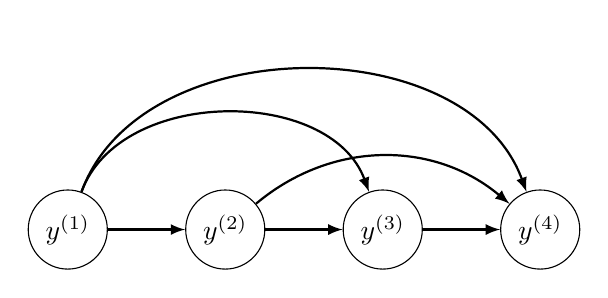
\begin{tikzpicture}[node distance=2cm,->,>=latex,auto,every edge/.append style={thick}]
	\node[state] (1) {$y^{(1)}$};
	\node[state] (2) [right of=1] {$y^{(2)}$};  
	\node[state] (3) [right of=2] {$y^{(3)}$};  
	\node[state] (4) [right of=3] {$y^{(4)}$};  
	
	\path(1) 
	edge[->] node{} (2)
	edge[bend left=70] node{} (3)
	edge[bend left=70] node{} (4);
	
	\path(2) 
	edge[->] node{} (3)
	edge[bend left=40] node{} (4);
	
	\path(3) edge[->] node{} (4);
	
	\end{tikzpicture}
\end{center}

If each value $y$ could take on the same fixed set of $k$ values, we would need to learn $k^4$ parameters to represent the joint distribution $P(\mathbb{Y})$. This clearly inefficient, since the number of parameters needed scales like $\mathcal{O}(k^\tau)$. If we relax the restriction that each $y^{(i)}$ must depend \textit{directly} on all past $y^{(j)}$, we can considerably reduce the number of parameters needed to compute the probability of some particular sequence. \\

\p We could include latent variables $h$ at each timestep that capture the dependencies, reminiscent of a classic RNN:

\begin{center}
	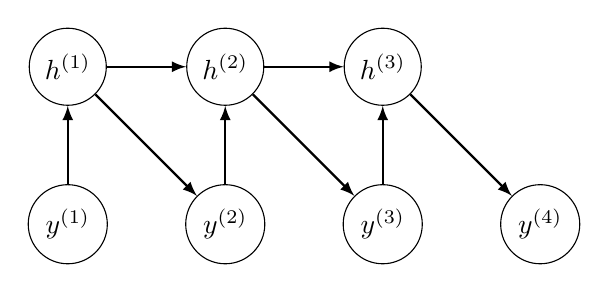
\begin{tikzpicture}[node distance=2cm,->,>=latex,auto,every edge/.append style={thick}]
	\node[state] (1) {$y^{(1)}$};
	\node[state] (2) [right of=1] {$y^{(2)}$};  
	\node[state] (3) [right of=2] {$y^{(3)}$};  
	\node[state] (4) [right of=3] {$y^{(4)}$};  
	
	\node[state] (h1) [above of=1]{$h^{(1)}$};
	\node[state] (h2) [above of=2]{$h^{(2)}$};
	\node[state] (h3) [above of=3]{$h^{(3)}$};
	
	\path(1) 	edge[->] node{} (h1);
	\path(2) 	edge[->] node{} (h2);
	\path(3) 	edge[->] node{} (h3);
	
	\path(h1) 	edge[->] node{} (h2)
	edge[->] node{} (2);
	
	\path(h2) 	edge[->] node{} (h3)
	edge[->] node{} (3);
	
	\path(h3) 	edge[->] node{} (4);
	\end{tikzpicture}
\end{center}
Since in the RNN case all factors $P(h^{(t)} \mid h^{(t-1)})$ are deterministic, we don't need any additional parameters to compute this probability\footnote{Don't forget that, in a neural net, a variable $y^{(t)}$ is represented by a \textit{layer}, which itself is composed of $k$ nodes, each associated with one of the $k$ unique values that $y^{(t)}$ could be.}, other than the single $m^2$ parameters needed to convert any $h^{(t)}$ to the next $h^{(t+1)}$ (which is shared across all transitions). Now, the number of parameters needed as a function of sequence length is constant, and as a function of $k$ is just $\mathcal{O}(k)$. \\

Finally, to view the RNN as a graphical model, we must describe how to sample from it, namely how to sample a sequence $\vec{y}$ from $P(\mathbb{Y})$, if parameterized by our graphical model above. In the general case where we don't know the value of $\tau$ for our sequence $\vec{y}$, one approach is to have a EOS symbol that, if found during sampling, means we should stop there. Also, in the typical case where we actually want to model $P(y \mid x)$ for input sequence $x$, we can reinterpret the parameters $\vec{\theta}$ of our graphical model as a function of $\vec{x}$ the input sequence. In other words, the graphical model interpretation becomes a function of $\vec{x}$, where $\vec{x}$ determines the exact values of the probabilities the graphical model takes on -- an ``instance'' of the graphical model.






\myspace
\p \blue{Bidirectional RNNs}. In many applications, it is desirable to output a prediction of $\vec{y}^{(t)}$ that may depend on \textit{the whole sequence}. For example, in speech recognition, the interpretation of words/sentences can also depend on what is \textit{about} to be said. Below is a typical bidirectional RNN, where the inputs $\vec{x}^(t)$ are fed both to a ``forward'' RNN ($\vec{h}$) and a ``backward'' RNN ($\vec{g}$). \marginnote{Notice how the output units $\vec{o}^{(t)}$ have the nice property of depending on both the past and future while being most sensitive to input values around time $t$.}[5em]

\myfig[0.3\textwidth]{BiRNN.PNG}

\myspace\myspace\Needspace{15\baselineskip}
\p \blue{Encoder-Decoder Seq2Seq Architectures (10.4)} Here we discuss how an RNN can be trained to map an input sequence to output sequence which is not necessarily the same length. (Not really much of a discussion...figure below says everything.)

\myfig{Seq2Seq.PNG}

\myspace\myspace\Needspace{15\baselineskip}
% --------------------------------------------
\subsub{Challenge of Long-Term Deps. (10.7)}
% --------------------------------------------

\myspace
\p Gradients propagated over many stages either vanish (usually) or explode. We saw how this could occur when we took parameter gradients earlier, and for weight matrices $\matr{W}$ further along from the loss node, the expression for $\matgrad{L}{W}$ contained multiplicative Jacobian factors. Consider the (linear activation) repeated function composition of an RNN's hidden state in \ref{10.36}. We can rewrite it as a power method (\ref{10.37}), and if $\matr{W}$ admits an eigendecomposition (remember $\matr{W}$ is necessarily square here), we can further simplify as seen in ~\ref{10.38}.\marginnote{\red{Q}: Explain interp. of mult. $\vec{h}$ by $\matr{Q}$ as opposed to the usual $\matr{Q}^T$ explained in the linear algebra review.}[2em]
\begin{align}
	\vec{h}^{(t)} &= \matr{W}^T \vec{h}^{(t-1)} \tlab{10.36} \\
	&= (\matr{W}^t)^T \vec{h}^{(0)} \tlab{10.37} \\
	&= \matr{Q}^T \matr{\Lambda}^t \matr{Q} \vec{h}^{(0)} \tlab{10.38}
\end{align}
\begin{quote}
	\textbf{Any component of $\vec{h}^{(0)}$ that isn't aligned with the largest eigenvector will eventually be discarded.}\footnote{Make sure to think about this from the right perspective. The largest value of $t = \tau$ in the RNNs we've seen would correspond with either (1) the largest output sequence or (2) the largest input sequence (if fixed-vector output). After we extract the output from a given forward pass, we reset the clock and either back-propagate errors (if training) or get ready to feed another sequence.}
\end{quote}
If, however, we have a non-recurrent network such that the state elements are repeatedly multiplied by different $w^{(t)}$ at each time step, the situation is different. Suppose the different $w^{(t)}$ are i.i.d. with mean 0 and variance $v$. The variance of the product is easily seen to be $\mathcal{O}(v^n)$\footnote{Quick sketch of (my) proof: \begin{align}
	 \Var{w^{(i)}} 
		 &= v 
			 = \E{(w^{(i)})^2} - \cancel{\E{w^{(i)}}^2} \\ 
	\Var{ \prod_t^n  w^{(t)}  } 
		&= \E{
			\left(
			\prod_t^n w^{(t)}
			\right)^2} 
		= \prod_t^n \E{  (    w^{ (t) }   )^2  } = v^n
	\end{align}}. \textit{To obtain some desired variance $v^*$ we may choose the individual weights with variance} $v = \sqrt[n]{v^*}$. 

\myspace\myspace\Needspace{15\baselineskip}
% --------------------------------------------
\subsub{LSTMs and Other Gated RNNs (10.10)}
% --------------------------------------------

\p While leaky units have connection weights that are either manually chosen constants or are trainable parameters, gated RNNs generalize this to connection weights that may change \textit{at each time step}. Furthermore, gated RNNs can learn to both accumulate and \textit{forget}, while leaky units are designed for just accumulation\footnote{Q: Isn't choosing to update with higher relative weight on the present the same as forgetting? A: Sort of. It's like ``soft forgetting'' and will inevitably erase more/less than desired (smeary). In this context, ``forget'' means to set the weight of a specific past cell to zero.}

\myspace
\p \blue{LSTM (10.10.1)}. The idea is we want self-loops to produce paths where the gradient can flow for long durations. The self-loop weights are \textbf{gated}, meaning they are controlled by another hidden unit, interpreted as being conditioned on \textit{context}. Listed below are the main components of the LSTM architecture.
\begin{compactitem}
	\item \textbf{Forget gate $f_i^{(t)} 
		= \sigma\left(b_i^f + \sum_j U_{i,j}^f x_j^{(t)} + \sum_j W_{i,j}^f h_j^{(t-1)}    \right)
		$}. \marginnote{The subscript, $i$, identifies the cell. The superscript, $t$, denotes the time.}
	
	\item \textbf{Internal state} $s_i^{(t)}
		= f_i^{(t)} \odot s_i^{(t-1)} + g_i^{(t)} \odot \sigma\left(b_i + \sum_j U_{i,j} x_j^{(t)} + \sum_j W_{i,j} h_j^{(t-1)}  \right)
		$. 
	
	\item \textbf{External input gate} $g_i^{(t)}
	= \sigma\left(b_i^g + \sum_j U_{i,j}^g x_j^{(t)} + \sum_j W_{i,j}^g h_j^{(t-1)}    \right)
	$.
	
	\item \textbf{Output gate} $q_i^{(t)}
	= \sigma\left(b_i^o + \sum_j U_{i,j}^o x_j^{(t)} + \sum_j W_{i,j}^o h_j^{(t-1)}    \right)
	$. 
\end{compactitem}
The final hidden state can then be computed via
\begin{align}
	h_i^{(t)} &= \tanh(s_i^{(t)}) \odot q_i^{(t)}
\end{align}










\lecture{Modern Practices}{Applications (Ch. 12)}{February 14}

\myspace

\subsub{Natural Language Processing (12.4)}

\marginnote{Begins on pg. 448}

\myspace
\p \blue{n-grams}. A \textbf{language model} defines a probability distribution over sequences of [discrete] tokens (words/characters/etc). Early models were based on the \textit{n-gram}: a [fixed-length] sequence of $n$ tokens. Such models define the conditional distribution for the $n$th token, given the $(n - 1)$ previous tokens: $$P(x_t \mid x_{t - (n - 1)}, \ldots, x_{t - 1})$$where $x_i$ denotes the token at step/index/position $i$ in the sequence. \\

\p To define distributions over longer sequences, we can just use Bayes rule over the shorter distributions, as usual. For example, say we want to find the [joint] distribution for some $\tau$-gram ($\tau > n$), and we have access to an $n$-gram model and a [perhaps different] model for the initial sequence $P(x_1, \ldots, x_{n - 1})$. We compute the $\tau$ distribution simply as follows:
\begin{align}
	P(x_1, \ldots, x_\tau) &= P(x_1, \ldots, x_{n - 1}) \prod_{t = n}^{\tau} 
		P(x_t \mid x_{t - 1}, \ldots, x_{t - (n - 2)}, x_{t - (n - 1)}) \tlab{12.5}
\end{align}
where it's important to see that each factor in the product is a distribution over a length-$n$ sequence. Since we need that initial factor, it is common to train both an $n$-gram model and an $n-1$-gram model simultaneously. \\

\p Let's do a specific example for a trigram (n = 3). 
\begin{compactitem}
	\item \textbf{Assumptions [for this trigram model example]}:
	\begin{compactitem}
		\item For any $n \ge 3$, $P(x_n \mid x_1, \ldots, x_{n - 1}) = P(x_n \mid x_{n - 2}, x_{n - 1})$. 
		
		\item When we get to computing the full joint distribution over some sequence of arbitrary length, we assume we have access to both $P_3$ and $P_2$, the joint distributions over all subsequences of length 3 and 2, respectively. 
	\end{compactitem}
	
	\item \textbf{Example sequence}: We want to know how to use a trigram model on the sequence ['THE', 'DOG', 'RAN', 'AWAY']. 
	
	\item \textbf{Derivation}: We can use the built-in model assumption to derive the following formula.
	\newcommand\fml[1]{\text{\footnotesize#1}}
	\begin{align}
	\begin{split}
		P(\fml{THE DOG RAN AWAY})
			&= P_3(\fml{AWAY} \mid \fml{THE DOG RAN})  ~ P_3(\fml{THE DOG RAN})\\
			&=  P_3(\fml{AWAY} \mid \fml{DOG RAN})  ~ P_3(\fml{THE DOG RAN})\\
			&= \frac{ P_3(\fml{DOG RAN AWAY}) }{ P_2(\fml{DOG RAN}) }  ~ P_3(\fml{THE DOG RAN})\\
			&= P_3(\fml{THE DOG RAN}) P_3(\fml{DOG RAN AWAY}) / P_2(\fml{DOG RAN})
	\end{split}\tlab{12.7}
	\end{align}
\end{compactitem}
\myspace
\p \blue{Limitations of n-gram}. The last example illustrates some potential problems one may encounter that arise [if using MLE] when the full joint we seek is nonzero, but (a) some $P_n$ factor is zero, or (b) $P_{n - 1}$ is zero\marginnote{Recall that, in MLE, the $P_n$ and $P_{n - 1}$ are usually approximated via counting occurrences in the training set}[-2em]. Some methods of dealing with this are as follows.
\begin{compactitem}
	\item \textbf{Smoothing}: shifting probability mass from the observed tuples to unobserved ones that are similar.
	\item \textbf{Back-off methods}: look up the lower-order (lower values of $n$) $n$-grams if the frequency of the context $x_{t - 1}, \ldots, x_{t - (n - 1)}$ is too small to use the higher-order model.
\end{compactitem}
In addition, $n$-gram models are vulnerable to the curse of dimensionality, since most $n$-grams won't occur in the training set\footnote{For a given vocabulary, which usually has much more than $n$ possible words, consider how many possible sequences of length $n$.}, even for modest $n$.


% =========================================
\subsub{Neural Language Models (12.4.2)}
% =========================================

\p Designed to overcome curse of dimensionality by using a distributed representation of words. Recognize that any model trained on sentences of length $n$ and then told to generalize to new sentences [also of length $n$] must deal with a space\footnote{Ok I tried re-wording that from the book's confusing wording but that was also a bit confusing. Let me break it down. Say you train on a thousand sentences each of length 5. For a given vocabulary of size VOCAB\_SIZE, the number of possible sequences of length 5 is $(\text{VOCAB\_SIZE})^5$, which can be quite a lot more than a thousand (not to mention the possibility of duplicate training examples). To the naive model, all points in this high-dimensional space are basically the same. A neural language model, however, tries to arrange the space of possibilities in a meaningful way, so that an unforeseen sample at test time can be said "similar" as some previously seen training example. It does this by \textit{embedding} words/sentences in a lower-dimensional feature space.} of possible sentences that is exponential in $n$. Such word representations (i.e. viewing words as existing in some high-dimensional space) are often called \textbf{word embeddings}. The idea is to map the words (or sentences) from the raw high-dimensional [vocab sized] space to a smaller feature space, where similar words are closer to one another. Using distributed representations may also be used with graphical models (think Bayes' nets) in the form multiple \textit{latent variables}. 










% ==================================================================================
% DEEP LEARNING RESEARCH
% ==================================================================================
\mysection{Deep Learning Research}\label{Deep Learning Research}

\lecture{Deep Learning Research}{Linear Factor Models (Ch. 13)}{January 12}

\myspace
\p \blue{Overview}. Much research is in building a \textit{probabilistic model}\footnote{Whereas, before, we've been building \textit{functions} of the input (deterministic).} of the input, $p_{model}(x)$. Why? Because then we can perform \textit{inference} to predict stuff about our environment given any of the other variables. We call the other variables \textbf{latent variables}, $h$, with
\begin{align}
	p_{model}(x) &= \sum_h \Pr(h)\Pr(x \mid h) = \mathbb{E}_h\left[ p_{model}(x \mid h)\right]
\end{align}
So what? Well, the latent variables provide another means of \textit{data representation}, which can be useful. \textbf{Linear factor models} (LFM) are some of the simplest probabilistic models with latent variables.
\begin{quote}
	A linear factor model is defined by the use of a stochastic linear decoder function that generates $\vec{x}$ by adding noise to a linear transformation of $\vec{h}$. 
\end{quote}
Note that $\vec{h}$ is a \textit{vector} of arbitrary size, where we assume $p(\vec{h})$ is a \purple{factorial distribution}: $p(\vec{h}) = \prod_i p(h_i)$. This roughly means we assume the elements of $\vec{h}$ are mutually independent\footnote{Note that, technically, this assumption isn't strictly the definition of mutual independence, which requires that every \textit{subset} (i.e. not just the full set) of $\{h_i \in \vec{h}\}$ follow this factorial property.}. The LFM describes the data-generation process as follows:
\begin{compactenum}
	\item Sample the explanatory factors: $\vec{h} \sim p(\vec{h})$.
	\item Sample the real-valued observable variables given the factors:
	
	\graybox{
		\vec{x} = \matr{W} \vec{h} + \vec{b} + \textrm{noise}
		}
\end{compactenum}

\myspace
\p \blue{Probabilistic PCA and Factor Analysis}.
\begin{compactitem}
	\item \textbf{Factor analysis}: 
	\begin{align}
		\vec{h} &\sim \mathcal{N}(\vec{h}; \vec{0}, \matr{I}) \\
		\text{noise} &\sim \mathcal{N}(\vec{0}, \vec{\psi}\equiv\text{diag}(\vec{\sigma^2})) \\
		\vec{x} &\sim \mathcal{N}(\vec{x};~ \vec{b}, \matr{W}\matr{W}^T + \vec{\psi})
	\end{align}
	where the last relation can be shown by recalling that a linear combination of Gaussian variables is itself Gaussian, and showing that $\mathbb{E}_h\left[\vec{x}\right] = \vec{b}$, and $\text{Cov}(\vec{x}) = \matr{W}\matr{W}^T + \vec{\psi}$. \\
	
	\p It is worth emphasizing the interpretation of $\vec{\psi}$ as the matrix of \green{conditional variances} $\sigma_i^2$. \textit{Huh?} Let's take a step back. The fact that we were able to separate the distributions in the above relations for $\vec{h}$ and $\text{noise}$ is from a built-in \underline{assumption} that $\Pr(x_i | \vec{h}, x_{j \ne i}) = \Pr(x_i | \vec{h})$\footnote{Due to $<$\textsc{math}$>$, this introduces a constraint that knowing the value of some element $x_j$ doesn't alter the probability $\Pr(x_i = W_i \cdot h + b_i + \text{noise})$. Given how we've defined the variable $\vec{h}$, this means that knowing $\text{noise}_j$ provides no clues about $\text{noise}_i$. Mathematically, the noise must have a diagonal covariance matrix.}. \\
	
	\redbox[The Big Idea]{
		The latent variable $\vec{h}$ is a big deal because it \textbf{captures the dependencies} between the elements of $\vec{x}$. \textit{How do I know?} Because of our assumption that the $x_i$ are conditionally independent given $\vec{h}$. If, once we specify $\vec{h}$, all the elements of $\vec{x}$ become independent, then any information about their interrelationship is hiding somewhere in $\vec{h}$.
	}
	\vspace{0.3em}
	Detailed walkthrough of Factor Analysis (a.k.a me slowly reviewing, months after taking this note):
	{\small
	\begin{compactitem}
		\item \textbf{Goal}. Analyze and understand the motivations behind how Factor Analysis defines the data-generation process under the framework of LFMs (defined in steps 1 and 2 earlier). Assume $\vec{h}$ has dimension $n$. 
		\item \textbf{Prior}. Defines $p(\vec{h}) := \mathcal{N}(\vec{h}; \vec{0}, \matr{I})$, the unit-variance Gaussian. Explicitly,
			$$
				p(\vec{h}) := \frac{1}{(2\pi)^{n/2}} e^{-\frac{1}{2} \sum_i^n h_i^2}
			$$
		\item \textbf{Noise}. Assumed to be drawn from a Gaussian with diagonal covariance matrix $\matr{\psi} := \diag{\vec{\sigma}^2}$. Explicitly,
		$$
			p(\text{noise} = \vec{a}) := \frac{1}{ (2\pi)^{n / 2} \prod_i^n \sigma_i } e^{-\frac{1}{2} \sum_i^n a_i^2 / \sigma_i^2}
		$$
		
		\item \textbf{Deriving distribution of $\vec{x}$}. We use the fact that any linear combination of Gaussians is itself Gaussian. Thus, deriving $p(\vec{x})$ is reduced to computing it's mean and covariance matrix.
		\begin{align}
			\vec[x]{\mu} &= \E[\vec{h}]{\matr{W} \vec{h} + \vec{b}} \\
			&= \int p(\vec{h}) (\matr{W} \vec{h} + \vec{b}) \mathrm{d}\vec{h} \\
			&= \vec{b} + \int \frac{1}{(2\pi)^{n/2}} e^{-\frac{1}{2} \sum_i^n h_i^2} \matr{W} \vec{h} \mathrm{d}\vec{h} \\
			&= \vec{b} \\
			\text{Cov}(\vec{x}) &= \E{(\vec{x} - \E{\vec{x}}) (\vec{x} - \E{\vec{x}})^T} \\
			&= \E{(\matr{W}\vec{h} + \text{noise})(\vec{h}^T \matr{W}^T + \text{noise}^T)} \\
			&= \E{(\matr{W}\vec{h}\vec{h}^T\matr{W}^T)} + \matr{\psi} \\
			&= \matr{W}\matr{W}^T + \matr{\psi}
		\end{align}
		where we compute the expectation of $\vec{x}$ over $\vec{h}$ because $\vec{x}$ is defined as a function of $\vec{h}$, and noise is always expectation zero.
		\item \textbf{Thoughts}. Not really seeing why this is useful/noteworthy. Feels very contrived (many assumptions) and restrictive -- it only applies if the dependencies between each $x_i$ can be modeled with a random variable $\vec{h}$ sampled from a unit variance Gaussian.
	\end{compactitem}}
	
	
	
	\vspace{0.3em}
	\item \textbf{Probabilistic PCA}: Just factor analysis with $\vec{\psi} = \sigma^2 \matr{I}$. So zero-mean spherical Gaussian noise. It becomes regular PCA as $\sigma \rightarrow 0$. Here we can use an iterative EM algorithm for estimating the parameters $\matr{W}$. 
\end{compactitem}

%
% AUTOENCODERS
% 
\lecture{Deep Learning Research}{Autoencoders (Ch. 14)}{May 07}

\p \blue{Introduction}. An autoencoder learns to copy its input to its output, via an encoder function $\vec{h} = f(\vec{x})$ and a decoder function $\vec{r} = g(\vec{h})$\marginnote{$\vec{r}$ for ``reconstruction''}. Modern autoencoders generalize this to allow for stochastic mappings $p_{encoder}(\vec{h} \mid \vec{x})$ and $p_{decoder}(\vec{x} \mid \vec{h})$.

\myspace
\p \blue{Undercomplete Autoencoders}. Constrain dimension of $\vec{h}$ to be smaller than that of $\vec{x}$. The learning process minimizes some $L(\vec{x}, g(f(\vec{x})))$, where the loss function could be e.g. mean squared error. Be careful not to have too many learnable parameters in the functions $g$ and $f$ (thus increasing model capacity), since that defeats the purpose of using an undercomplete autoencoder in the first place.

\myspace
\p \blue{Regularized Autoencoders}. We can remove the undercomplete constraint/necessity by modifying our loss function. For example, a \green{sparse autoencoder} one that adds a penalty $\Omega(\vec{h})$ to the loss function that encourages the \textit{activations on} (not connections to/from) the hidden layer to be sparse. One way to achieve \textit{actual zeros} in $\vec{h}$ is to use rectified linear units for the activations.


%
% AUTOENCODERS
% 
\lecture{Deep Learning Research}{Representation Learning (Ch. 15)}{May 07}

\myspace
\p \blue{Greedy Layer-Wise Unsupervised Pretraining}. Given:
\begin{compactitem}[-]
	\item Unsupervised learning algorithm $\mathcal{L}$ which accepts as input a training set of examples $\matr{X}$, and outputs an encoder/feature function $f$. 
	\item $f^{(i)}(\matr{\tilde{X}})$ denotes the output of the $i$th layer of $f$, given as \textit{immediate input} the (possibly transformed) set of examples $\matr{\tilde{X}}$.
	\item Let $m$ denote the number of layers (``stages'') in the encoder function (note that each layer/stage here \textit{must} use a representation learning algorithm for its $\mathcal{L}$ e.g. an RBM, autoencoder, sparse coding model, etc.)
\end{compactitem}
The procedure is as follows:
\begin{compactenum}
	\item Initialize.
	\begin{align}
		f(\cdot) &\leftarrow I(\cdot) \\
		\tilde{\matr{X}} &= \matr{X}
	\end{align}
	
	\item For each layer (stage) $i$ in $\text{range}(m)$, do:
	\begin{align}
		f^{(k)} &= \mathcal{L}(\tilde{\matr{X}}) \\
		f(\cdot) &\leftarrow  f^{(k)}\left(f\left(\cdot\right)\right) \\
		\tilde{\matr{X}} &\leftarrow f^{(k)}(\tilde{\matr{X}})
	\end{align}
	In English: just apply the regular learning/training process for each layer/stage \textbf{sequentially and individually}\footnote{In other words, you proceed one layer at a time \textit{in order}. You don't touch layer $i$ until the weights in layer $i - 1$ have been learned.}.
\end{compactenum}
When this is complete, we can run \green{fine-tuning}: train all layers together (including any later layers that could not be pretrained) with a supervised learning algorithm. Note that we do indeed allow the pretrained encoding stages to be optimized here (i.e. not fixed).

% 
% PROBABILISTIC MODELS
% 
\lecture{Deep Learning Research}{Structured Probabilistic Models for DL (Ch. 16)}{October 01, 2017}

\p \blue{Motivation}. In addition to classification, we can ask probabilistic models to perform other tasks such as density estimation ($\vec{x} \rightarrow p(\vec{x})$), denoising, missing value imputation, or sampling. What these [other] tasks have in common is they require a \textit{complete understanding of the input}. Let's start with the most naive approach of modeling $p(\vec{x})$, where $\vec{x}$ contains $n$ elements, each of which can take on $k$ distinct values: we store a lookup table of all possible $\vec{x}$ and the corresponding probability value $p(\vec{x})$. This requires $k^n$ parameters\footnote{Consider the common NLP case where our vector $\vec{x}$ contains $n$ word tokens, each of which can take on any symbol in our vocabulary of size $v$. If we assign $n=100$ and $v=100,000$, which are relatively common values for this case, this amounts to $(1e5)^{1e2} = 10^{500}$ parameters.}. Instead, we use graphs to describe model structure (direct/indirect interactions) to drastically reduce the number of parameters.

\myspace
\p \blue{Directed Models}. Also called \green{belief networks} or \green{Bayesian networks}. Formally, a directed graphical model defined on a set of variables $\{\vec{x}\}$ is defined by a DAG, $\mathcal{G}$, whose vertices are the random variables in the model, and a set of \textbf{local conditional probability distributions}, $p(x_i \mid Pa_{\mathcal{G}}(x_i))$, where $Pa_{\mathcal{G}}(x_i)$ gives the parents of $x_i$ in $\mathcal{G}$. The probability distribution over $\vec{x}$ is given by
\graybox{
	p(\vec{x}) = \prod_i p(x_i \mid Pa_{\mathcal{G}}(x_i))
	}
	
\myspace
\p \blue{Undirected Graphical Models}. Also called \green{Markov Random Fields (MRFs)} or \green{Markov Networks}. Appropriate for situations where interactions do not have a well-defined direction. Each \green{clique} $\mathcal{C}$ (any set of nodes that are all [maximally] connected) in $\mathcal{G}$ is associated with a factor $\phi(\mathcal{C})$. The factor $\phi(\mathcal{C})$, also called a \green{clique potential}, is just a function (not necessarily a probability) that outputs a number when given a possible set of values over the nodes in $\mathcal{C}$. The output number measures the affinity of the variables in that clique for being in the states specified by the inputs\marginnote{Clique potentials are constrained to be nonnegative.}[-2em]. The set of all factors in $\mathcal{G}$ defines an \textbf{unnormalized probability distribution}:
\graybox{
	\widetilde{p}(\vec{x}) = \prod_{\mathcal{C} \in \mathcal{G}} \phi(\mathcal{C})
	}

\myspace
\p \blue{The Partition Function}. To obtain a valid probability distribution, we must normalize the probability distribution:
\begin{align}
	p(\vec{x}) &= \frac{1}{Z} \widetilde{p}(\vec{x}) \\
	Z &= \int \widetilde{p}(\vec{x}) \mathrm{d}\vec{x}
\end{align}
where the normalizing function $Z = Z(\{\phi\})$ is known as the \green{partition function} (physicz sh0ut0uT). It is typically intractable to compute, so we resort to approximations. Note that $Z$ isn't even guaranteed to exist -- it's only for those definitions of the clique potentials that cause the integral over $\widetilde{p}(\vec{x})$ to converge/be defined.

\myspace
\p \blue{Energy-Based Models} (EBMs). A convenient way to enforce $\forall \vec{x}, ~ \widetilde{p}(\vec{x}) > 0$ is to use EBMs, where
\begin{align}
	\widetilde{p}(\vec{x}) \triangleq \exp\left( -E(\vec{x}) \right)
\end{align}
and $E(\vec{x})$ is known as the \green{energy function}\footnote{Physics throwback: this mirrors the Boltzmann factor, $\exp(-\varepsilon/\tau)$, which is proportional to the probability of the system being in quantum energy state $\varepsilon$.}. Many algorithms need to compute not $p_{model}(\vec{x})$ but only $\log\widetilde{p}_{model}(\vec{x})$ (unnormalized log probabilities - logits!). For EBMs with latent variables $\vec{h}$, such algorithms are phrased in terms of the \green{free energy}:
\begin{align}
	\mathcal{F}(\vec{x} = x) &= -\log \sum_{h} \exp\left( - E(\vec{x}=x, ~ \vec{h} = h ) \right)
\end{align}
where we sum over all possible assignments of the latent variables.


\myspace
\p \blue{Separation and D-Separation}. We want to know which subsets of variables are conditionally independent from each other, given the values of other subsets of variables.  A set of variables $\mathbb{A}$ is \green{separated} (if undirected model)/\green{d-separated} (if directed model) from another set of variables $\mathbb{B}$ given a third set of variables $\mathbb{S}$ if the graph structure implies that $\mathbb{A}$ is independent from $\mathbb{B}$ given $\mathbb{S}$. 

\begin{compactitem}
	\item \green{Separation}. For \textit{undirected} models. If variables $a$ and $b$ are connected by a path involving only \underline{unobserved} variables (an \green{active} path), then $a$ and $b$ are \textit{not} separated. Otherwise, they are separated. Any paths containing at least one observed variable are called \green{inactive}.

	\item \green{D-Separation}\footnote{The D stands for dependence.}. For \textit{directed} models. Although there are rules that help determine whether a path between $a$ and $b$ is d-separated, it is simplest to just determine whether $a$ is independent from $b$ given any observed variables along the path.
\end{compactitem}


% ------------------------------------------------
\myspace\Needspace{18\baselineskip}
\subsub{Sampling from Graphical Models}
\myspace
% ------------------------------------------------

\p For directed graphical models, we can do \green{ancestral sampling} to produce a sample $\vec{x}$ from the joint distribution represented by the model. Just sort the variables $x_i$ into a topological ordering such that $\forall i,j: j > i \iff x_i \in Pa_{\mathcal{G}}(x_j)$. To produce the sample, just sequentially sample from the beginning, $x_1 \sim P(x_1)$, $x_2 \sim P(x_2 \mid Pa_{\mathcal{G}}(x_1) )$, etc.\\

\p For undirected graphical models, one simple approach is \green{Gibbs sampling}. Essentially, this involves drawing a conditioned sample from $x_i \sim p(x_i \mid \text{neighbors}(x_i))$ for each $x_i$. This process is repeated many times, where each subsequent pass uses the previously sampled values in $\text{neighbors}(x_i)$ to obtain an asymptotically converging [to the correct distribution] estimate for a sample from $p(\vec{x})$.

% ------------------------------------------------
\myspace\Needspace{18\baselineskip}
\subsub{Inference and Approximate Inference}
\myspace
% ------------------------------------------------

\p One of the main tasks with graphical models is predicting the values of some subset of variables given another subset: inference. Although the graph structures we've discussed allow us to represent complicated, high-dimensional distributions with a reasonable number of parameters, the graphs used for deep learning are usually not restrictive enough to allow efficient inference. \green{Approximate inference} for deep learning usually refers to variational inference, in which we approximate the distribution $p(\vec{h} \mid \vec{v})$ by seeking an approximate distribution $q(\vec{h} \mid \vec{v})$ that is as close to the true one as possible. 

\myspace
\p \blue{Example: Restricted Boltzmann Machine}. The quintessential example of how graphical models are used for deep learning. The canonical RBM is an energy-based model with \textbf{binary} visible and hidden units. Its energy function is
\graybox{
	E(\vec{v}, \vec{h}) &= -\vec{b}^T\vec{v} - \vec{c}^T\vec{h} - \vec{v}^T\matr{W}\vec{h}
	}
where $\vec{b}$, $\vec{c}$, and $\matr{W}$ are unconstrained, real-valued, learnable parameters. One could interpret the values of the bias parameters as the affinities for the associated variable being its given value, and the value $\matr[i,j]{W}$ as the affinity of $v_i$ being its value and $h_j$ being its value at the same time\footnote{More concretely, remember that $\vec{v}$ is a one-hot vector representing some state that can assume len($\vec{v}$) unique values, and similarly for $\vec{h}$. Then $\matr[i,j]{W}$ gives the affinity for the state associated with $v$ being its $i$th value \textit{and} the state associated with $h$ being its $j$th value.}. \\

The restrictions on the RBM structure, namely the fact that there are no intra-layer connections, yields nice properties. Since $\widetilde p(\vec{h},\vec{v})$ can be factored into clique potentials, we can say that:
\begin{align}
	p(\vec{h} \mid \vec{v}) &= \prod_i p(h_i \mid \vec{v}) \\
	p(\vec{v} \mid \vec{h}) &= \prod_i p(v_i \mid \vec{h})
\end{align}
Also, due to the restriction of binary variables, each of the conditionals is easy to compute, and can be quickly derived as
\begin{align}
	p(h_i = 1 \mid \vec{v}) &= \sigma\left( c_i + \vec{v}^T\matr[:,i]{W} \right)
\end{align}
allowing for efficient block Gibbs sampling. 



%
% MONTE CARLO METHODS
% 
\lecture{Deep Learning Research}{Monte Carlo Methods (Ch. 17)}{May 09}

\p \blue{Monte Carlo Sampling (Basics)}. We can approximate the value of a (usually prohibitively large) sum/integral by viewing it as an \textit{expectation} under some distribution. We can then approximate its value by taking samples from the corresponding probability distribution and taking an empirical average. Mathematically, the basic idea is show below:
\graybox{
	s = \int p(\vec{x}) f(\vec{x}) \mathrm{d}\vec{x} = \E[p]{f(\rvec{x})}
	\quad\rightarrow\quad
	\hat{s}_n = \frac{1}{n} \sum_{i = 1,~\rvec{x}^{(i)} \sim p}^{n} f(\vec{x}^{(i)})
}
As we've seen before, the empirical average is an unbiased\footnote{
	Recall that expectations on such an average are still taken over the underlying (assumed) probability distribution:
	\begin{align}
		\E[p]{\hat{s}_n} &= \frac{1}{n} \sum_{i = 1}^{n} \E[p]{f(\vec{x}^{(i)})} \\
		&= \frac{1}{n} \sum_{i = 1}^{n} s \\
		&= s
	\end{align}
	You should think of the expectation $\E[p]{f(\vec{x}^{(i)})}$ as the expected value of the \textit{random sample} from the underlying distribution, which of course is $s$, because we defined it that way. 
	} estimator. Furthermore, the central limit theorem tells us that the distribution of $\hat{s}_n$ converges to a normal distribution with mean $s$ and variance $\Var{f(\vec{x})}/n$. 
	
\myspace
\p \blue{Importance Sampling}. What if it's not feasible for us to sample from $p$? We can approach this a couple ways, both of which will exploit the following identity:
\begin{align}
	p(\vec{x}) f(\vec{x}) = q(\vec{x}) \frac{p(\vec{x}) f(\vec{x})}{q(\vec{x})}
\end{align}
\begin{itemize}
	\item \textbf{Optimal importance sampling}. We can use the aforementioned identity/decomposition to find the \green{optimal $q*$} -- optimal in terms of number of samples required to achieve a given level of accuracy. First, we rewrite our estimator $\hat{s}_p$ (they now use subscript to denote the sampling distribution) as $\hat{s}_q$:
	\begin{align}
		\hat{s}_q &=  \frac{1}{n} \sum_{i = 1,~\rvec{x}^{(i)} \sim q}^{n} \frac{p(\vec{x}^{(i)}) f(\vec{x}^{(i)})}{q(\vec{x}^{(i)})}
	\end{align}
	At first glance, it feels a little wonky, but recognize that we are \textit{sampling from q instead of p} (i.e. if this were an integral, it would be over $q(\vec{x})\mathrm{d}\vec{x}$). The catch is that, now, the variance can be greatly sensitive to the choice of $q$:
	\begin{align}
		\Var{\hat{s}_q} &= \Var{\frac{p(\vec{x}) f(\vec{x})}{q(\vec{x})}} / n
	\end{align}
	with the optimal (minimum) value of $q$ at:
	\graybox{
		q* &= \frac{p(\vec{x})\mid f(\vec{x}) \mid}{Z}
		}
		
	\item \textbf{Biased importance sampling}. Computing the optimal value of $q$ can be as challenging/infeasible as sampling from $p$. Biased sampling does not require us to find a normalization constant for $p$ or $q$. Instead, we compute:
	\begin{align}
		\hat{s}_{BIS} &= \dfrac{
			\sum_{i = 1}^{n} \frac{\tilde p(\vec{x}^{(i)})}{\tilde q(\vec{x}^{(i)})}  f(\vec{x}^{(i)})
			}{
			\sum_{i = 1}^{n} \frac{\tilde p(\vec{x}^{(i)})}{\tilde q(\vec{x}^{(i)})}  
			}
	\end{align}
	where $\tilde p$ and $\tilde q$ are the unnormalized forms of $p$ and $q$, and the $\vec{x}^{(i)}$ samples are still drawn from [the original/unknown] $q$. $\E{\hat s_{BIS}} \ne s$ except asymptotically when $n \rightarrow \infty$. 
\end{itemize}







%
% Confronting the Partition Function
% 
\lecture{Deep Learning Research}{Confronting the Partition Function (Ch. 18)}{August 30, 2018}



\p \blue{Noise Contrastive Estimation} (NCE) (18.6). We now estimate
\begin{align}
	\log p_{model}(\vec x)
		&= \log \tilde{p}_{model}(\vec x; \vec\theta) + c
\end{align}
and explicitly learn an approximation, $c$, for $-\log Z(\vec\theta)$. Obviously MLE would just try jacking up $c$ to maximize this, so we adopt a surrogate supervised training problem: binary classification that a given sample $\vec x$ belongs to the (true) data distribution $p_{data}$ or to the noise distribution $p_{noise}$. We introduce binary variable $y$ to indicate whether the sample is in the true data distribution ($y{=}1$) or the noise distribution ($y{=}0$). Our surrogate model is thus defined by
\begin{align}
	p_{joint}(y{=}1) &= \onehalf \\
	p_{joint}(\vec x \mid y{=}1) &= p_{model}(\vec x) \\
	p_{joint}(\vec x \mid y{=}0) &= p_{noise}(\vec x) 
\end{align}
We can now use MLE on the optimization problem,
\graybox{
	\vec\theta , c 
		&= \argmax_{\vec\theta , c} \E[\vec x, y \sim p_{train}]{\log p_{joint}(y \mid \vec x)} \\
	p_{joint}(y{=}1 \mid \vec x)
		&= \frac{  p_{model}(\vec x) }{  p_{model}(\vec x) + p_{noise}(\vec x) } \\
		&= \inv{  1 + p_{noise}(\vec x) / p_{model}(\vec x)  } \\
		&= \sigma\left(  
			\log p_{model}\left( \vec x \right) -
			\log p_{noise}\left( \vec x \right)
		\right)
}

































%
% APPROXIMATE INFERENCE
% 
\lecture{Deep Learning Research}{Approximate Inference (Ch. 19)}{Nov 15, 2017}

% log(p(v; theta))
\newcommand\lpv{\log p(\vec{v}; \vec{\theta})}
\renewcommand\elbo{\mathcal{L}(\vec v, \vec{\theta}, q)}
\newcommand\Dkl[2]{D_{KL}\left( #1 ~||~ #2 \right)}

\p \blue{Overview}. Most graphical models with multiple layers of hidden variables have intractable posterior distributions. This is typically because the partition function scales exponentially with the number of units and/or due to marginalizing out latent variables. Many approximate inference approaches make use of the observation that exact inference can be described as an optimization problem. \\ 

Assume we have a probabilistic model consisting of observed variables $\vec{v}$ and latent variables $\vec{h}$. We want to compute $\log p(\vec v;\vec{\theta})$, but it's too costly to marginalize out $\vec{h}$. Instead, we compute a lower bound $\mathcal{L}(\vec v, \vec{\theta}, q)$ -- often called the \green{evidence lower bound} (ELBO) or negative \green{variational free energy} -- on $\log p(\vec v; \vec{\theta})$\footnote{Recall that $D_{KL}(P || Q) = \E[x \sim P(x)]{\log \frac{P(x)}{Q(x)} }$}:\marginnote{$q$ is an arbitrary probability distribution over $\vec{h}$. Note that the book will write $q$ when they really mean $q(\vec h \mid \vec v)$.}[2em]
\graybox{
	\elbo &= \lpv - \Dkl{ q(\vec{h} \mid \vec{v}) }{p(\vec{h} \mid \vec{v}; \vec{\theta})} \\
	&= - \E[\vec{h} \sim q(\vec h \mid \vec v)]{\log p(\vec h, \vec v)} + H(q(\vec h \mid \vec v))
}
where the second form is the more canonical definition\footnote{This can be derived easily from the first form. Hint: $$
	\log \frac{q(\vec h \mid \vec v)}{ p(\vec h \mid \vec v)} = 
	\log \frac{q(\vec h \mid \vec v)}{ p(\vec h, \vec v; \vec{\theta}) / p(\vec v; \vec{\theta})} 
$$}. Note that $\elbo$ is a lower-bound on $\lpv$ by definition, since 
$$\lpv - \elbo = D_{KL}\left(q(\vec{h} \mid \vec{v}) ||
p(\vec{h} \mid \vec{v}; \vec{\theta}) \right) \ge 0
$$
With equality (to zero) iff $q$ is the same distribution as $p(\vec h \mid \vec v)$. In other words, $\mathcal L$ can be viewed as a function parameterized by $q$ that's maximized when $q$ is $p(\vec h \mid \vec v)$, and with maximal value $\log p(\vec v)$. Therefore, we can cast the \textit{inference} problem of computing the (log) probability of the observed data  $\log p(\vec v)$ into an \textit{optimization} problem of maximizing $\mathcal L$. Exact inference can be done by searching over a family of functions that contains $p(\vec h \mid \vec v)$. 

\myspace
\p \blue{Expectation Maximization} (19.2). Technically not an approach to approximate inference, but rather an approach to learning with an approximate posterior. Popular for training models with latent variables. The EM algorithm consists of alternating between the followi[p]ng 2 steps until convergence:
\begin{compactenum}
	\item \textbf{E-step}. For each training example $\vec{v}^{(i)}$ (in current batch or full set), set
	\begin{align}
		q(\vec{h} \mid \vec{v}^{(i)}  )
			&= p(\vec{h} \mid \vec{v}^{(i)}; \vec{\theta}^{(0)})
	\end{align}
	where $\vec{\theta}^{(0)}$ denotes the current parameter values of the model at the beginning of the E-step. This can also be interpreted as maximizing $\mathcal L$ w.r.t. $q$. 
	
	\item \textbf{M-step}. Update the parameters $\vec{\theta}$ by completely or partially finding
	\begin{align}
		\argmax_{\vec{\theta}} \sum_i \mathcal{L}\left(\vec{v}^{(i)}, \vec{\theta}, q(\vec{h} \mid \vec{v}^{(i)}; \vec{\theta}^{(0)} ) \right)
	\end{align} 
\end{compactenum}













%
% APPROXIMATE INFERENCE
% 
\lecture{Deep Learning Research}{Deep Generative Models (Ch. 20)}{July 28, 2018}


\p \blue{Boltzmann Machines} (20.1). An energy-based model over a $d$-dimensional binary random vector $\rvec{x} \in \{0, 1\}^d$. The energy function is simply $E(\vec{x}) = -\vec{x}^T \matr U \vec x - \vec{b}^T \vec x$, i.e. parameters between all pairs of $x_i, x_j$, and bias parameters for each $x_i$\footnote{Authors are being lazy because it's assumed the reader is familiar (which is fair, I guess). i.e. they aren't mentioning that this formula implies that $\matr U$ is either lower or upper triangular, and the diagonal is zero.}. In settings where our data consists of samples of fully observed $\vec x$, this is clearly limited to very simple cases, since e.g. the probability of some $x_i$ being on is given by logistic regression from the values of the other units. 

\begin{example}[Proof: prob of \(x_i\) being on is logistic regression on other units]
	\tiny
	It's important to be as specific as possible here, since the task stated as-is is ambiguous. We want to prove that the probability of some fully observed state $\vec x$ that has its $i$th element clamped to $1$, which I'll denote as $p_{i=on}(\vec x)$, is logistic regression over the other units.\\
	
	To prove this, it's easier to use the conventional definition where $\matr U$ is symmetric with zero diagonal, and we write $E(\vec x)$ as
	\begin{align}
		E(\vec x)
			&= - \sum_{i=1}^{d} \sum_{j=i+1}^{d} x_i U_{i,j} x_j - \sum_{i=1}^{d} b_i x_i
	\end{align}
	where the difference is that we explicitly only sum over the upper triangle of $\matr U$. \\
	
	Intuitively, since $p(\{ \vec x \}_{j \ne i}) = p_{i=on}(\vec x) + p_{i=off}(\vec x)$, our final formula for $p_{i=on}$ should only contain terms involving the parameters that interact with $x_i$, and only for those cases where $x_i=1$. This motivates exploring the formula for $\Delta E_i (\vec x) \triangleq E_{i=off} - E_{i=on}$ where I've dropped the explicit notation on $\vec x$ for simplicity/space. Before jumping in to deriving this, step back and realize that $\Delta E_i$ will only contain summation terms where either the row or column index of $\matr U$ is $i$, and only for terms with bias element $b_i$. Since our summation is over the upper triangle of $\matr U$, this means terms along the slices $U_{i, i+1:d}$ and $U_{1:i-1, i}$. Now there is no derivation needed and we can simply write
	\begin{align}
		\Delta E_i 
			&= \sum_{k = i + 1}^{d} U_{i, k} x_k + \sum_{k = 1}^{i-1} x_k U_{k, i} + b_i 
	\end{align}
	
	The goal is to use this to get a logistic-regression-like formula for $p_{i=on}$, so we should now think about the relationship between any given $p(\vec x)$ and the associated $E(\vec x)$. The critical observation is that $E(\vec x) = -\ln p(\vec x) - \ln Z$, which therefore means
	\begin{align}
		\Delta E_i
			&= \ln p_{i=on}(\vec x) - \ln p_{i=off}(\vec x)
			= - \ln\left( \frac{ 1 - p_{i=on}(\vec x)  }{p_{i=on}(\vec x)}  \right) \\
		\exp(- \Delta E_i)
			&=  \frac{ 1 - p_{i=on}(\vec x)  }{p_{i=on}(\vec x)} =  \frac{ 1 }{p_{i=on}(\vec x)} - 1 \\
		\therefore p_{i=on}(\vec x)
			&= \frac{ 1 }{ 1 +  \exp(- \Delta E_i) }
	\end{align}
	Since $\Delta E_i$ is a linear function of all other units, we have proven that $p_{i=on}(\vec x)$ for some state $\vec x$ reduces to logistic regression over the other units. 
\end{example}

\myspace
\p \blue{Restricted Boltzmann Machines} (20.2). A BM with variables partitioned into two sets: hidden and observed. The graphical model is bipartite over the hidden and observed nodes, as I've drawn in the example below. 
\begin{center}
	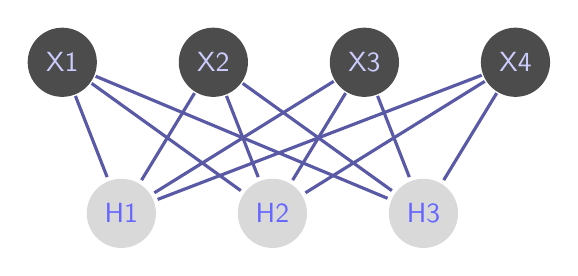
\begin{tikzpicture}[font=\sffamily,node distance=1.cm,->,>=latex,auto,line width=0.4mm]
	
	\tikzset{node st/.style={state, draw=none,
			fill=gray!30!white,
			text=blue!60!white}}
	\tikzset{node obs/.style={state, draw=none,
			fill=gray!60!black,
			text=blue!20!white}}
	
	\node[node obs] (X1) {X1};
	\node[node obs, right=of X1] (X2) {X2};
	\node[node obs, right=of X2] (X3) {X3};
	\node[node obs, right=of X3] (X4) {X4};
	
	\node[node st, below=of X1, xshift=0.75cm] (Y1) {H1};
	\node[node st, right=of Y1] (Y2) {H2};
	\node[node st, right=of Y2] (Y3) {H3};
	
	\draw[every loop,
	auto=right,
	draw=blue!30!gray]
	(X1) edge[-]				node{} (Y1)
	(X1) edge[-]				node{} (Y2)
	(X1) edge[-]				node{} (Y3)
	(X2) edge[-]				node{} (Y1)
	(X2) edge[-]				node{} (Y2)
	(X2) edge[-]				node{} (Y3)
	(X3) edge[-]				node{} (Y1)
	(X3) edge[-]				node{} (Y2)
	(X3) edge[-]				node{} (Y3)
	(X4) edge[-]				node{} (Y1)
	(X4) edge[-]				node{} (Y2)
	(X4) edge[-]				node{} (Y3);
	\end{tikzpicture}
\end{center}
Although the joint distribution $p(\vec x, \vec h)$ has a potentially intractable partition function, the conditional distributions can be computed efficiently by exploiting independencies:
\begin{align}
	p(\vec h \mid \vec x)
		&= \prod_{j = 1}^{n_h} \sigma \left( [2 \vec h - 1] \odot [\vec c + \matr{W}^T \vec x]    \right)_j \\
	p(\vec x \mid \vec h) 
		&= \prod_{i = 1}^{n_x} \sigma \left( [2 \vec x - 1] \odot [\vec b + \matr W \vec h]  \right)_i
\end{align}
where $\vec b$ and $\vec c$ are the observed and hidden bias parameters, respectively.

\myspace
\p \blue{Deep Belief Networks} (20.3). Several layers of (usually binary) latent variables and a single observed layer. The "deepest" (away from the observed) layer connections are undirected, and all other layers are directed and pointing toward the data. I've drawn an example below.

\begin{center}
	\scalebox{0.8}{
	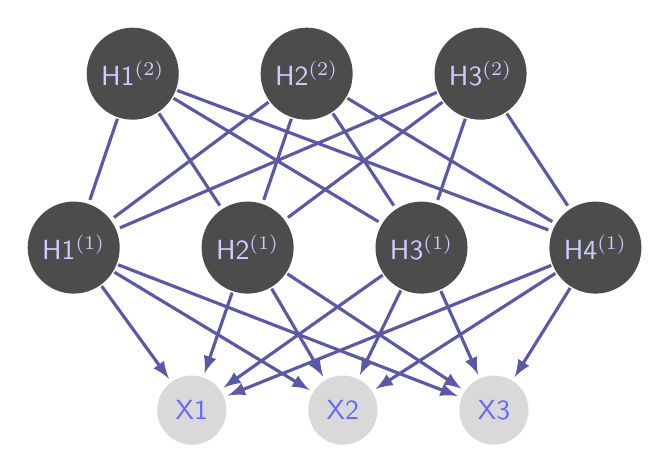
\begin{tikzpicture}[font=\sffamily,node distance=1.cm,->,>=latex,auto,line width=0.4mm]
	
	\tikzset{node st/.style={state, draw=none,
			fill=gray!30!white,
			text=blue!60!white}}
	\tikzset{node obs/.style={state, draw=none,
			fill=gray!60!black,
			text=blue!20!white}}
	
	\node[node obs] (X1) {H1$^{(2)}$};
	\node[node obs, right=of X1] (X2) {H2$^{(2)}$};
	\node[node obs, right=of X2] (X3) {H3$^{(2)}$};
	
	\node[node obs, below=of X1, xshift=-0.75cm] (X11) {H1$^{(1)}$};
	\node[node obs, right=of X11] (X21) {H2$^{(1)}$};
	\node[node obs, right=of X21] (X31) {H3$^{(1)}$};
	\node[node obs, right=of X31] (X41) {H4$^{(1)}$};	
	
	\node[node st, below=of X11, xshift=1.5cm] (Y1) {X1};
	\node[node st, right=of Y1] (Y2) {X2};
	\node[node st, right=of Y2] (Y3) {X3};

	
	\foreach \o in {X11, X21, X31, X41} {
		\foreach \i in {X1, X2, X3} {
			\draw[every loop, auto=right, blue!30!gray] (\i) edge[-] (\o) ; 
		};
	} ;
	
	\foreach \o in {Y1, Y2, Y3} {
		\foreach \i in {X11, X21, X31, X41} {
			\draw[every loop, auto=right, blue!30!gray] (\i) edge[->] (\o);
		};	
	};
	
	\end{tikzpicture}}
\end{center}
We can sample from a DBN via first Gibbs sampling on the undirected layer, then ancestral sampling through the rest of the (directed) model to eventually obtain a sample from the visible units.

\myspace 
\p \blue{Deep Boltzmann Machines} (20.4). Same as DBNs, but now all layers are undirected. Note that this is very close to the standard RBM, since we have a set of hidden and observed variables, except now we interpret certain subgroups of hidden units as being in a ``layer'', thus allowing for connections between hidden units in adjacent layers. What's interesting is that this still defines a bipartite graph, with odd-numbered layers on one side and even on the other\footnote{Recall that this immediately implies that units in all odd layers are conditionally independent given the even layers (and vice-versa for even to odd).}. \\

\myspace
\p \blue{Differentiable Generator Networks} (20.10.2). Use a differentiable function $g(\vec z; \vec{\theta}^{(g)})$ to transform samples of latent variables $\rvec z$ to either (a) samples $\rvec x$, or (b) distributions over samples $\rvec x$. For an example of case (a), the standard procedure for sampling from $\mathcal N(\vec\mu, \matr\Sigma)$ is to first sample from $\mathcal{N}(\vec 0, \matr I)$ into a generator network consisting of a single affine layer:\marginnote{\textbf{Case a}: interpret $g(\vec z)$ as emitting $\vec x$ directly.}[-1em]
$$
	\vec x \leftarrow g(\vec z) = \vec{\mu} + \matr L \vec z
$$
where $\matr L$ is the \textit{Cholesky decomposition}\footnote{The [unique] Cholesky decomposition of a (real-symmetric) p.d. matrix $\matr A$ is a decomposition of the form $\matr A = \matr L \matr L^T$, where $\matr L$ is lower triangular.} of $\matr\Sigma$. In general, we think of the generator function $g$ as providing a change of variables that transforms the distribution over $\rvec z$ into the desired distribution $\rvec x$. Of course, there \textit{is} an exact formula for doing this,
\begin{align}
	p_x(\vec x) 
		&= \frac{ p_z(g^{-1}(\vec x))  }{  \left|  \det \pderiv{g}{\vec z}  \right| }
\end{align}
but it's usually far easier to use indirect means of learning $g$, rather than trying to maximize/evaluation $p_x(\vec x)$ directly. \\

For case (b), the common approach is to train the generator net to emit conditional probabilities\marginnote{\textbf{Case b}: interpret $g(\vec z)$ as emitting $p(\vec x \mid \vec z)$.}[0em]
\begin{align}
	p(x_i \mid \vec z) = g(\vec z)_i \qquad\qquad p(\vec x) = \E[\vec z]{p(\vec x \mid \vec z)}
\end{align}
which can also support generating discrete data (case a cannot). The challenge in training generator networks is that we often have a set of examples $\vec x$, but the value of $\vec z$ for each $\vec x$ is not fixed and known ahead of time. We'll now look at some ways of training generator nets given only training samples for $\vec x$. Note that such a setting is very unlike unsupervised learning, where we typically interpret $\vec x$ as inputs that we don't have labels for, while here we interpret $\vec x$ as \textit{outputs} that we don't know the associated inputs for. 

\myspace 
\p \blue{Variational Autoencoders} (20.10.3). VAEs are directed models that use learned approximate inference and can be trained purely with gradient-based methods. To generate a sample $\vec x$, the VAE first samples $\vec z$ from the \textit{code distribution} $p_{model}(\vec z)$. This sample is then fed through the a differentiable generator network $g(\vec z)$. Finally, $\vec x$ is sampled from $p_{model}(\vec x; g(\vec z)) = p_{model}(\vec x \mid \vec z)$.  

\end{document}








